%% ****** Start of file aiptemplate.tex ****** %
%%
%%   This file is part of the files in the distribution of AIP substyles for REVTeX4.
%%   Version 4.1 of 9 October 2009.
%%
%
% This is a template for producing documents for use with 
% the REVTEX 4.1 document class and the AIP substyles.
% 
% Copy this file to another name and then work on that file.
% That way, you always have this original template file to use.


\documentclass[aip,graphicx]{revtex4-1}
%\documentclass[aip,reprint]{revtex4-1}

\usepackage{graphicx} \usepackage[caption=false]{subfig}
\usepackage{array} \usepackage{amsmath} \usepackage{bm}
\usepackage{auto-pst-pdf} \usepackage{psfrag} \usepackage{pstricks}

\newcommand{\sym}[1]{\text{#1}} \newcommand{\dif}{\mathrm{d}}
\newcommand{\degree}[1]{#1 \: ^{\circ}} \newcommand{\degC}[1]{#1 \;
  ^{\circ} \text{C}} \newcommand{\degCpm}[2]{#1 \pm #2 \; ^{\circ}
  \text{C}} \newcommand{\pder}[2][]{\frac{\partial#1}{\partial#2}}
\newcommand{\der}[2][]{\frac{\text{d}#1}{\text{d}#2}}
\newcommand{\matder}[2][]{\frac{\text{D}#1}{\text{D}#2}}
\newcommand{\secondder}[2][]{\frac{\text{d}^2#1}{\text{d}#2}}
\newcommand{\vect}[1]{\bm{#1}}

\draft % marks overfull lines with a black rule on the right

\begin{document}

% Use the \preprint command to place your local institutional report number 
% on the title page in preprint mode.
% Multiple \preprint commands are allowed.
%\preprint{}

%\title{Influence of the film thickness on the spreading regimes of a viscous drop spreading on an identical film} %Title of paper
\title{Sinking, wedging, spreading -- viscous spreading on an
  identical layer}

% repeat the \author .. \affiliation  etc. as needed
% \email, \thanks, \homepage, \altaffiliation all apply to the current author.
% Explanatory text should go in the []'s, 
% actual e-mail address or url should go in the {}'s for \email and \homepage.
% Please use the appropriate macro for the type of information

% \affiliation command applies to all authors since the last \affiliation command. 
% The \affiliation command should follow the other information.

\author{Nico Bergemann} \author{Matthias Heil} \author{Anne Juel}
%\email[]{Your e-mail address}
%\homepage[]{Your web page}
%\thanks{}
%\altaffiliation{}
\affiliation{The University of Manchester}

% Collaboration name, if desired (requires use of superscriptaddress option in \documentclass). 
% \noaffiliation is required (may also be used with the \author command).
%\collaboration{}
%\noaffiliation

\date{\today}

\begin{abstract}
% insert abstract here
TO BE REVISED\\ We investigated experimentally and computationally the
viscous spreading of a sessile drop on an identical layer.  A
practical application of this process is spray coating during which
subsequent drops spread on an existing layer of the same fluid.  We
performed spreading experiments on a uniform layer as well as on a dry
substrate and characterised the driving forces in both cases.  In the
case of spreading on a layer the flow is governed by viscous forces,
whereas the spreading on a dry substrate is governed by surface
tension.  We then performed computational simulations of the drop
spreading on an identical layer using the finite element method (FEM),
as implemented in \texttt{oomph-lib}.  These computations showed
excellent agreement with the experiments.  Through further
computations we established distinct spreading regimes depending on
the thickness of the layer.  For very thick fluid layers the drop
primarily sinks into the layer instead of spreading radially.  On the
other hand, for very thin layers the drop spreads similarly to a drop
on dry substrate, where the spreading is governed by gravity.  For
intermediate layer thicknesses the drop spreads through an advancing
wedge which is sustained by fluid flow from the drop into the layer.
\end{abstract}

\pacs{}% insert suggested PACS numbers in braces on next line

\maketitle %\maketitle must follow title, authors, abstract and \pacs

% Body of paper goes here. Use proper sectioning commands. 
% References should be done using the \cite, \ref, and \label commands


\section{Introduction}
\label{sec:introduction}
%\subsection{}
%\subsubsection{}

\noindent TO BE WRITTEN\\ The spreading of liquids on solid substrates
has received a lot of attention among the research community
\cite{de1985wetting, bonn2009wetting}.  Another area of interest is
the spreading of a liquid on top of another (immiscible) liquid
\cite{fraaije1989dynamics, joos1977spreading}.  While these two
configurations of droplet spreading are well investigated, limited
research has been performed in the spreading of a sessile Newtonian
drop on a layer of the same fluid \cite{tanner1979spreading,
  cormier2012beyond, chebbi1999capillary}.  Here we investigate the
spreading of a Newtonian glucose syrup on a thick layer of the same
fluid and find that in this case the flow is governed by a competition
of viscous and gravitational forces.  Moreover, we show that for the
spreading on a solid substrate the well established spreading law of
$R \propto t^{1/10}$ is obtained, which describes flow which is
governed by a competition of surface tension and gravity
\cite{bonn2009wetting}.

\section{Experiments}
\label{sec:experiments}

\subsubsection{Experimental setup}
\label{sec:experimental_setup}

\begin{figure}[!h]
\centering
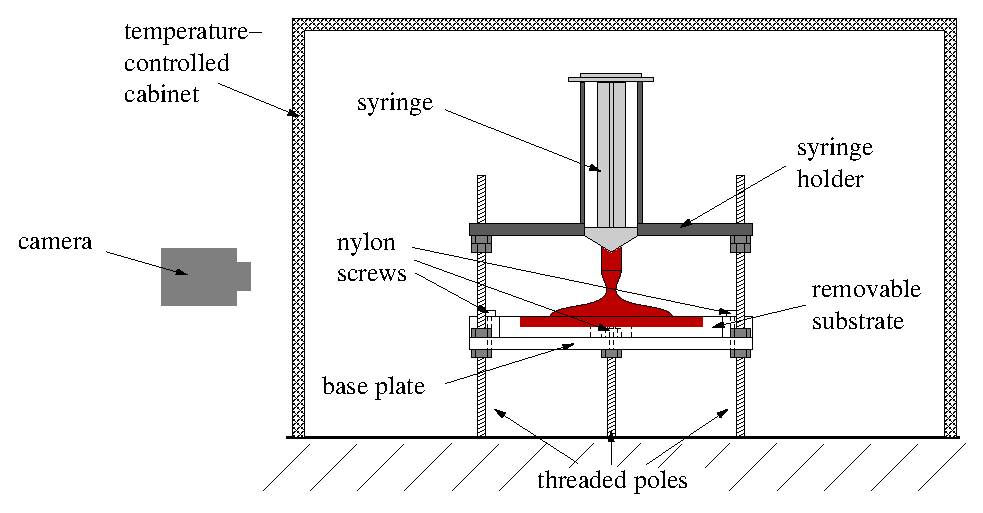
\includegraphics[width=0.99\textwidth]{figures/experimental_apparatus_updated.eps}
\caption{Schematic diagram of the experimental apparatus.}
\label{fig:experimental_apparatus}
\end{figure}

A schematic diagram of the experimental apparatus is
shown in Fig. \ref{fig:experimental_apparatus}. The substrate was
supported on a Perspex base plate, which was adjustably mounted on
three vertical, threaded poles (with a pitch of 1.25) using nuts, thus allowing accurate
levelling to $\pm 1^\circ$. The substrate (a Perspex plate of
dimensions $100 \times 100 \times 10$ mm with surfaces milled to an
accuracy of $\pm 0.02$ mm)
was secured to the base plate with three finger-tight nylon screws. A
featureless, flat substrate was used for the dry spreading
experiments, whereas for spreading on a viscous layer, a centred,
circular trough with a diameter of 60.5 mm and depth of 2 $\pm 0.02$ mm was milled into the plate. The fluid was deposited using a
standard 10 ml plastic syringe whose inner diameter was enlarged 
to 8 $\pm 0.05$ mm to facilitate the manual deposition of the high
viscosity liquid. To ensure reproducible deposition of the
fluid, we placed the syringe inside a tightly-fitting removable
holder which was mounted on the three vertical, threaded poles, 
allowing its level to be adjusted in a similar way to the base plate. The
accurate levelling of both base plate and syringe holder was essential
to ensure axisymmetric spreading. The working part of the experimental 
setup was enclosed in a temperature-controlled Perspex cabinet within which the 
temperature was held at $\degCpm{20.3}{0.2}$ {\bf *** NB: For the glucose
  experiments, I did not use the temperature control, although I performed the
  experiments in the cabinet. Instead I just recorded the (ambient lab) temperature
  for each experiment. So I'm not sure whether we should include the
  cabinet... ***  }.
Side-view images of the backlit drop were captured with a wall-mounted 
CCD camera (Pulnix TM-6740CL, 640x480 pixels). 

We performed the spreading experiments with glucose syrup (manufacturer: Cerestar UK Ltd.), which is a transparent, highly viscous Newtonian
liquid. In order to enhance contrast in the images, the glucose syrup
was dyed using red and green food colouring.  Mixing of the dye
entrained air bubbles, which were left to rise out of the fluid
overnight. The experiments were performed by filling the syringe with
5 ml of glucose syrup and wiping any excess fluid from the outside of
the nozzle with a dry paper towel. The filled syringe was then placed
inside the syringe holder, the image acquisition was initiated, and
the plunger of the syringe was displaced manually to empty the
syringe barrel within a deposition time of $2.4 \pm 0.5$ s.

We measured the density of the glucose syrup at the laboratory temperature
of $\degCpm{20.3}{0.2}$ to be $\rho=1372.8 \; \pm \; 4.9 \;
\sym{kg}/\sym{m}^3$ {\bf *** round off? NB: What do you mean by this? ***}  by accurately weighing five samples of known
volume between 10 and 50~ml.  The viscosity of glucose syrup depends
sensitively on temperature \cite{llewellin2002rheology} and we
therefore measured it at 20.0, 20.1, 20.3, 20.5 and $\degC{21.0}$
using a Brookfield R/S-Plus (SST) rheometer with a concentric cylinder
CC25 geometry and temperature control. We performed shear rate
measurements with linear increase from zero to a maximum value of $25
\; \sym{s}^{-1}$ with increments of $1 \; \sym{s}^{-1}$, applying a
cycle of incremental shear rate increase and decrease.  The total
experimentation time was 50 s, with one measurement taken every
second. Hence, for each temperature we recorded 50 viscosity
measurements and these experiments confirmed that the viscosity of
glucose syrup is independent of the shear rate and hence behaves as a
Newtonian fluid within the parameter range investigated. The resulting
averaged values of the dynamic viscosity $\mu$ are presented in table
\ref{tab:glucose_viscosity}, showing similar viscosities in the range
$20.0 - \degC{20.3}$, but a 7\% decrease at $\degC{21.0}$. The
laboratory temperature was recorded for each spreading experiment, so
that the viscosity could be inferred. 


{\renewcommand{\arraystretch}{1.2}
 \begin{table}[!ht]
 \begin{center}
 \begin{tabular}{c | c}
  Temperature in $\degC{}$ & Viscosity $\mu$ in Pa.s \\ \hline 20.0 &
  $43.62 \; \pm \; 0.22$ \\ 20.1 & $43.72 \; \pm \; 0.19$ \\ 20.3 &
  $43.61 \; \pm \; 0.23$ \\ 20.5 & $42.51 \; \pm \; 0.21$ \\ 21.0 &
  $40.34 \; \pm \; 0.19$\\
 \end{tabular}
 \caption{Viscosity measurements for glucose syrup at different
   temperatures.}
 \label{tab:glucose_viscosity}
 \end{center}
 \end{table}}


\subsubsection{Substrate preparation\label{sec:creating_layer}}
When performing the experiments in which the drop is 
deposited on a uniform layer of the same fluid, we prepared the
substrate by slightly overfilling the trough and then scraping
off the excess fluid with a square-edged ruler. 
This method is quick and therefore prevents the formation of a skin
due to evaporation and subsequent crystallisation at the surface \cite{lees2012sugar,edwards2000science}.
Since a certain amount of the (very viscous) fluid 
adhered to the scraper this procedure resulted in an underfilled trough, 
with the surface of the fluid layer located at a distance $\delta^*$ 
below the upper surface of the substrate, as illustrated in Fig. 
\ref{fig:axisym_drop_nozzle_gap}. While the thickness of the layer, 
$h^*$, was therefore smaller than the depth of the trough, the
process produced layers of very uniform thickness, with
$h^*$ varying by less than $\pm 4\%$ throughout the trough. 
The fact that the initial free surface was located below the
upper surface of the substrate meant that the outermost radius
of the propagating air-liquid interface that was observable by the camera,
$R_{z=0}(t)$, was smaller than the actual radius of the spreading front,
 $R_{z=-\delta^*}(t)$.
We will return to this issue in \S \ref{sec:comp_spreading_on_layer}.

\begin{figure}[!ht]
\centering
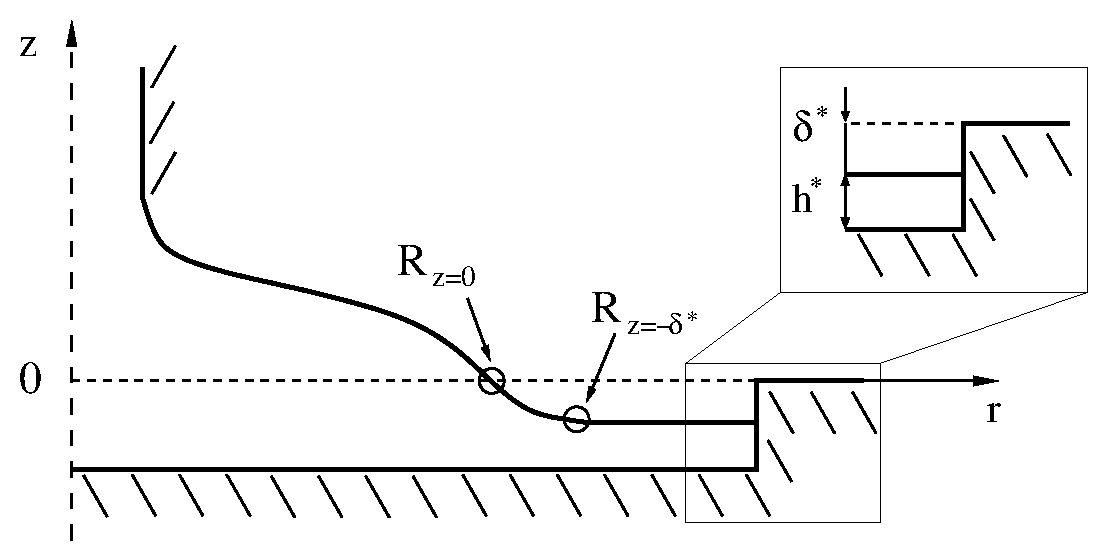
\includegraphics[width=0.7\textwidth]{figures/axisym_drop_nozzle_gap_updated.eps}
\caption{Schematic diagram of the underfilled trough, illustrating the
thickness of the layer $h^*$ and the distance to the upper surface of
the substrate $\delta^*$. Also specified in the schematic are the
radius as observed by the camera, $R_{z=0}$, and the actual radius of
the spreading front, $R_{z=-\delta^*}$.}
\label{fig:axisym_drop_nozzle_gap}
\end{figure}
 
\subsubsection{Image analysis\label{image}}
We analysed the images that were aquired by the camera using the \textit{OpenCV}
software \cite{bradski2008learning} within a \textit{python} environment.  In
order to convert the results from the image analysis into dimensional
quantities, a calibration image of a cylindrical object of known
dimensions was recorded prior to each experiment. This showed
that we achieved a spatial resolution of $0.111 \pm 0.006$
mm/pixel. Unavoidable small misalignment of the camera was corrected for in
post-processing by rotating the image prior to the analysis, so that
the platform edge was perfectly parallel to the image edge.
We recorded the spreading of the drop as a sequence of images, taken at a
rate of 20~fps and then analysed the resulting images over a period of 
15 s from the end of the initial drop deposition. In each image we determined 
the positions of the air-liquid interface, the upper edge of the
substrate and the end of the nozzle, using standard edge detection
routines.
We implemented these routines, which identify edges based on discontinuities in the
intensity profile of the image, in the \textit{OpenCV} framework.
Sub-pixed accuracy was achieved by exploiting the smooth variations 
in the intensity profile. 
We determined the position of the edge based on functional fits to the
intensity profile. In particular, we used tanh functions for solid
edges \cite{nalwa1986detecting}, such as the substrate and nozzle edges, and spline functions for
the air-liquid interface
\cite{poggio1985computational,poggio1988regularized}. The spline fit
proved necessary because the interface became increasingly diffuse as the
drop spread due to surface reflections. The robustness of
the analysis was improved by using the interface position detected in the
previous frame of the sequence as an initial condition. Hence, for all
images following the initial frame we applied the edge finding routine
to a region of $\pm$ 5 pixels horizontally and $\pm$ 2 pixels
vertically of the interface position located in the preceding
frame. We determined the coordinates of the air-liquid interface separately
for the left and right sides of each image. The radii obtained from
the two sides typically differed by less than 2\%, indicating that
the drops tended to spread very axisymmetrically. Representative
results obtained from our edge detection algorithms are shown in in Fig. 
\ref{fig:glucose_spreading} where the orange line indicates the lower
end of the nozzle, the green line the upper boundary of the 
substrate and the red line the air-liquid interface. The blue line
shows the nozzle centreline. The coordinates of the interface were 
measured relative to an $(r^*,z^*)$-coordinate system that was centered at
the intersection of the blue and green lines.


%\begin{figure}[!ht]
%\centering
%\includegraphics[trim={10px 150px 10px 75px},clip,width=0.5\textwidth]{figures/%111014_glucose_syrup_thick_layer_8_0117_analysed.eps}
%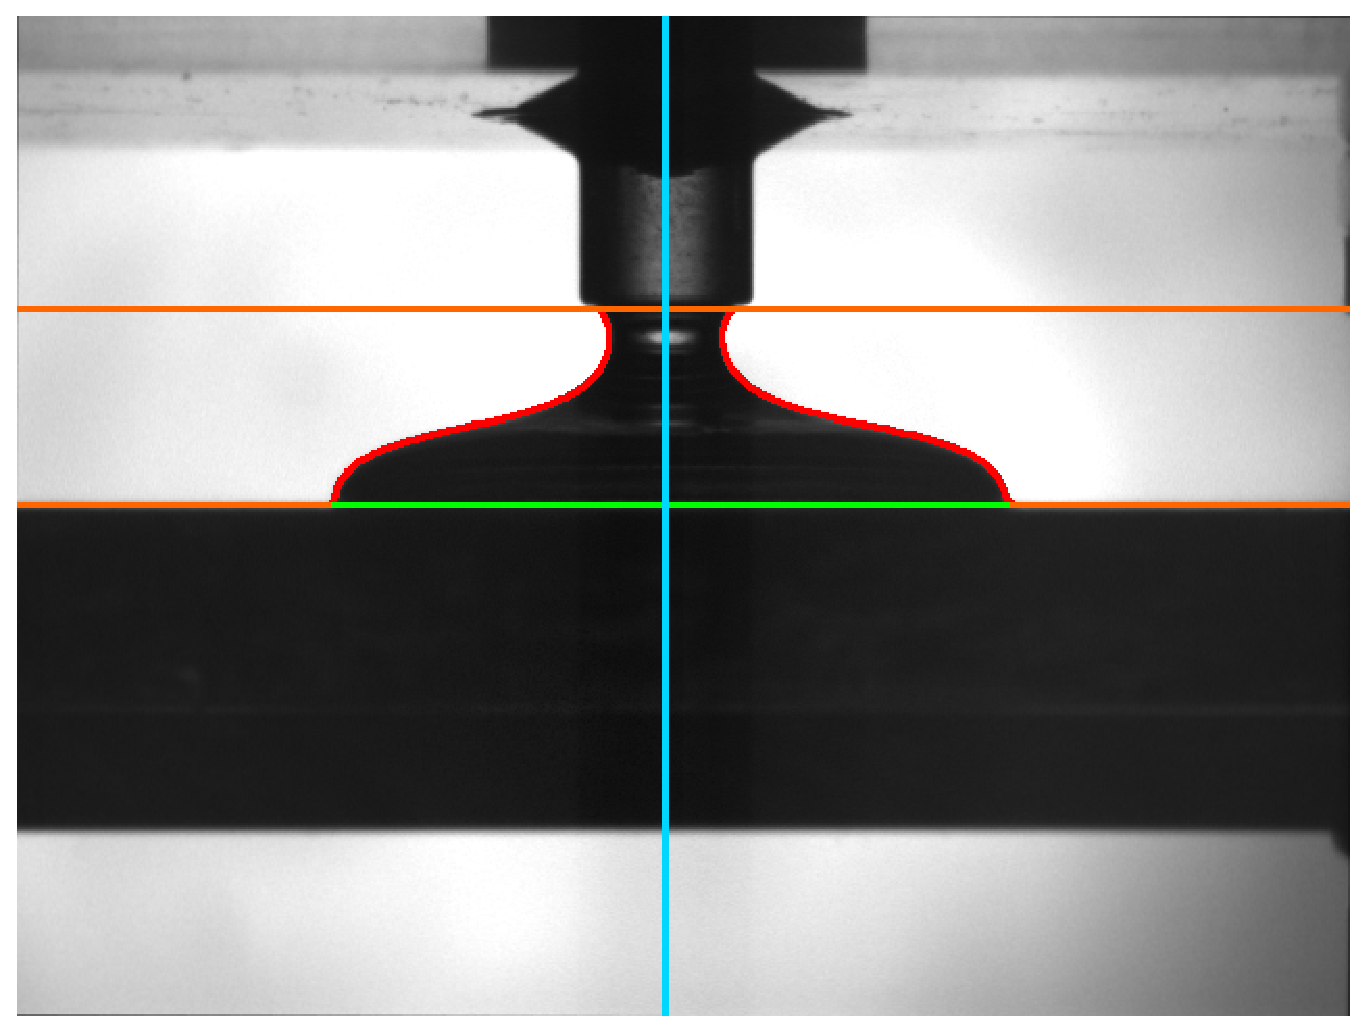
\includegraphics[clip,width=0.5\textwidth]{figures/111014_glucose_syrup_thick_layer_8_0117_analysed.eps}
%\caption{Example of image analysis: the nozzle centreline, the
%  platform edge and nozzle end, the drop diameter and free surface are
%  shown with cyan, orange, green and red lines, respectively.}
%\label{fig:analysis_glucose}
%\end{figure}

\subsection{Experimental results}
\label{sec:exp_results}

\begin{figure}[!ht]
 \captionsetup[subfloat]{position=top,singlelinecheck=false,
   margin=-0.5cm, justification=raggedright} \centering
 \subfloat[\label{fig:111014_glucose_syrup_dry_substrate_3_0100_analysed}]{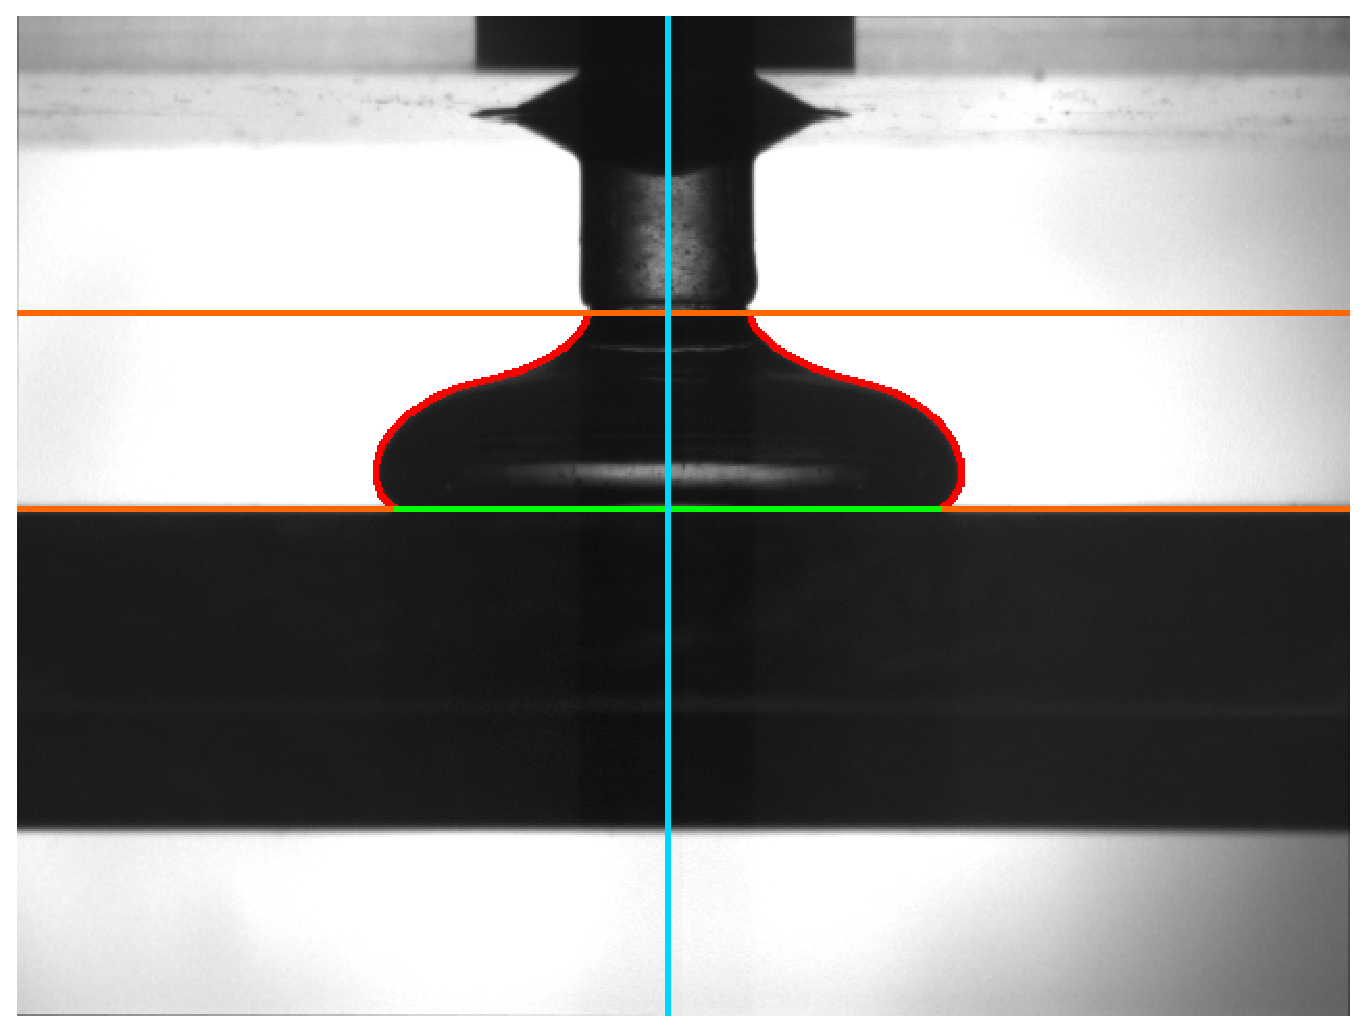
\includegraphics[trim={10px
       150px 10px
       75px},clip,width=0.4\textwidth]{figures/111014_glucose_syrup_dry_substrate_3_0100_analysed.eps}}\addtocounter{subfigure}{+3} \hspace{0.5cm}
 \subfloat[\label{fig:111014_glucose_syrup_thick_layer_8_0067_analysed}]{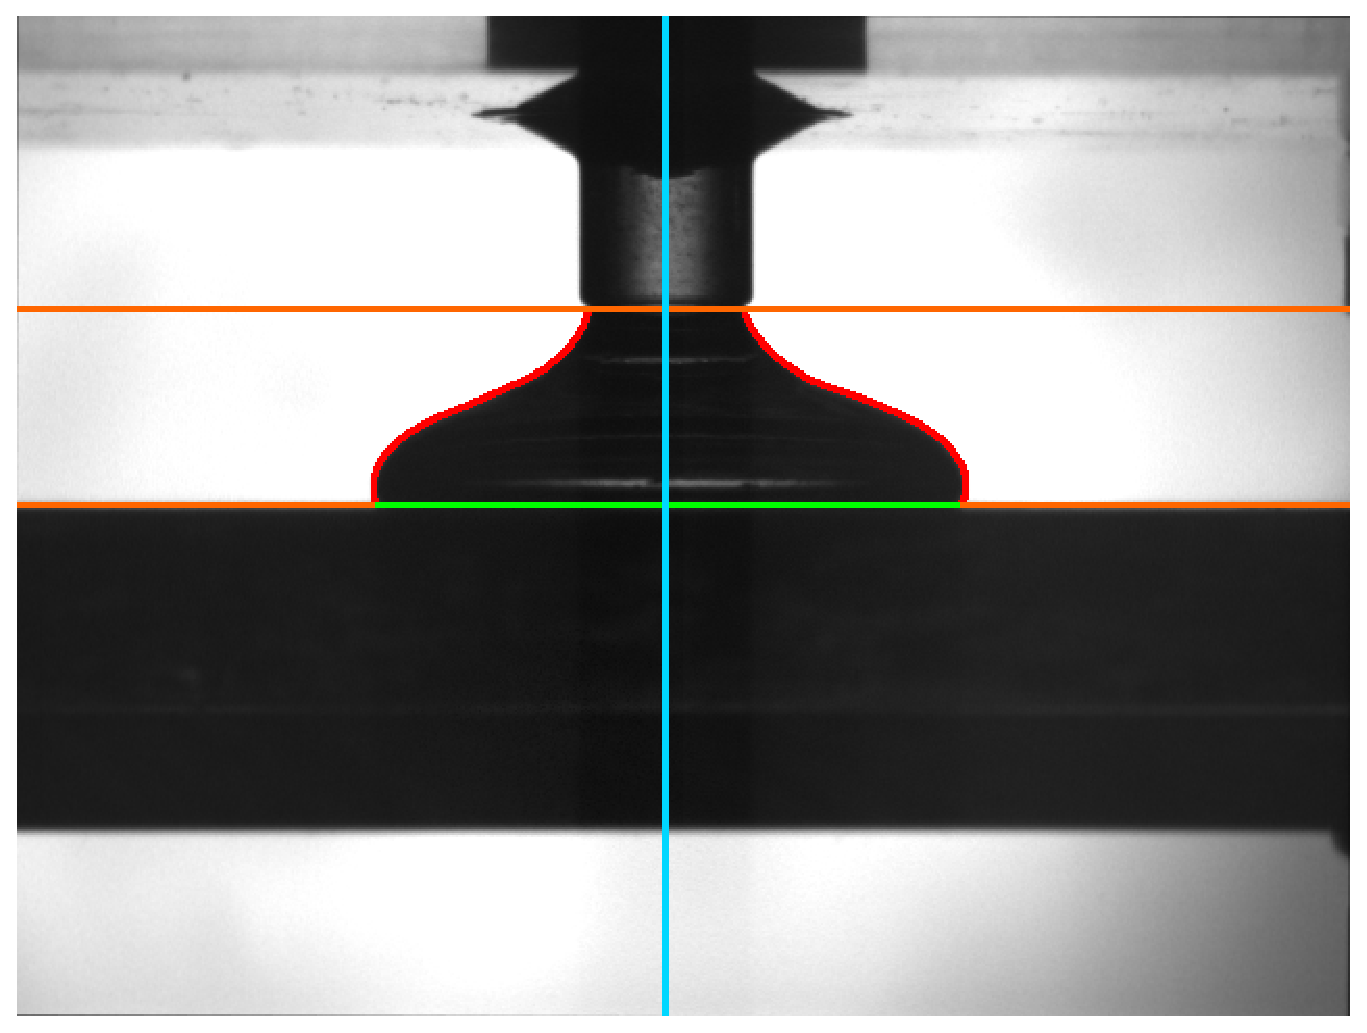
\includegraphics[trim={10px
       150px 10px
       75px},clip,width=0.4\textwidth]{figures/111014_glucose_syrup_thick_layer_8_0067_analysed.eps}}\addtocounter{subfigure}{-4}
 \\ \subfloat[\label{fig:111014_glucose_syrup_dry_substrate_3_0150_analysed}]{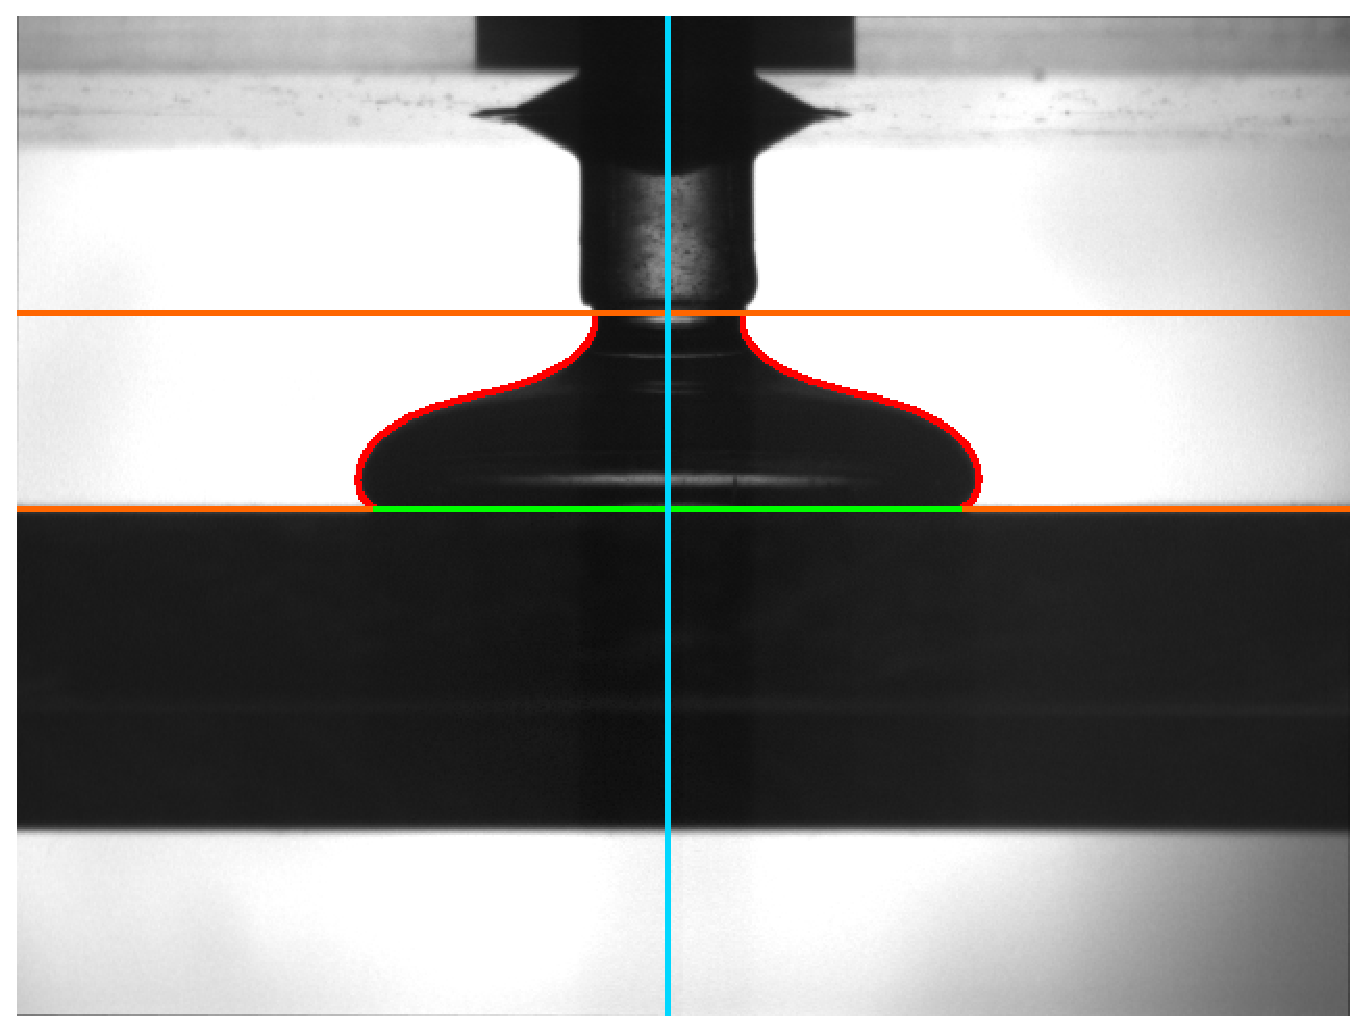
\includegraphics[trim={10px
       150px 10px
       75px},clip,width=0.4\textwidth]{figures/111014_glucose_syrup_dry_substrate_3_0150_analysed.eps}}\addtocounter{subfigure}{+3} \hspace{0.5cm}
 \subfloat[\label{fig:111014_glucose_syrup_thick_layer_8_0117_analysed}]{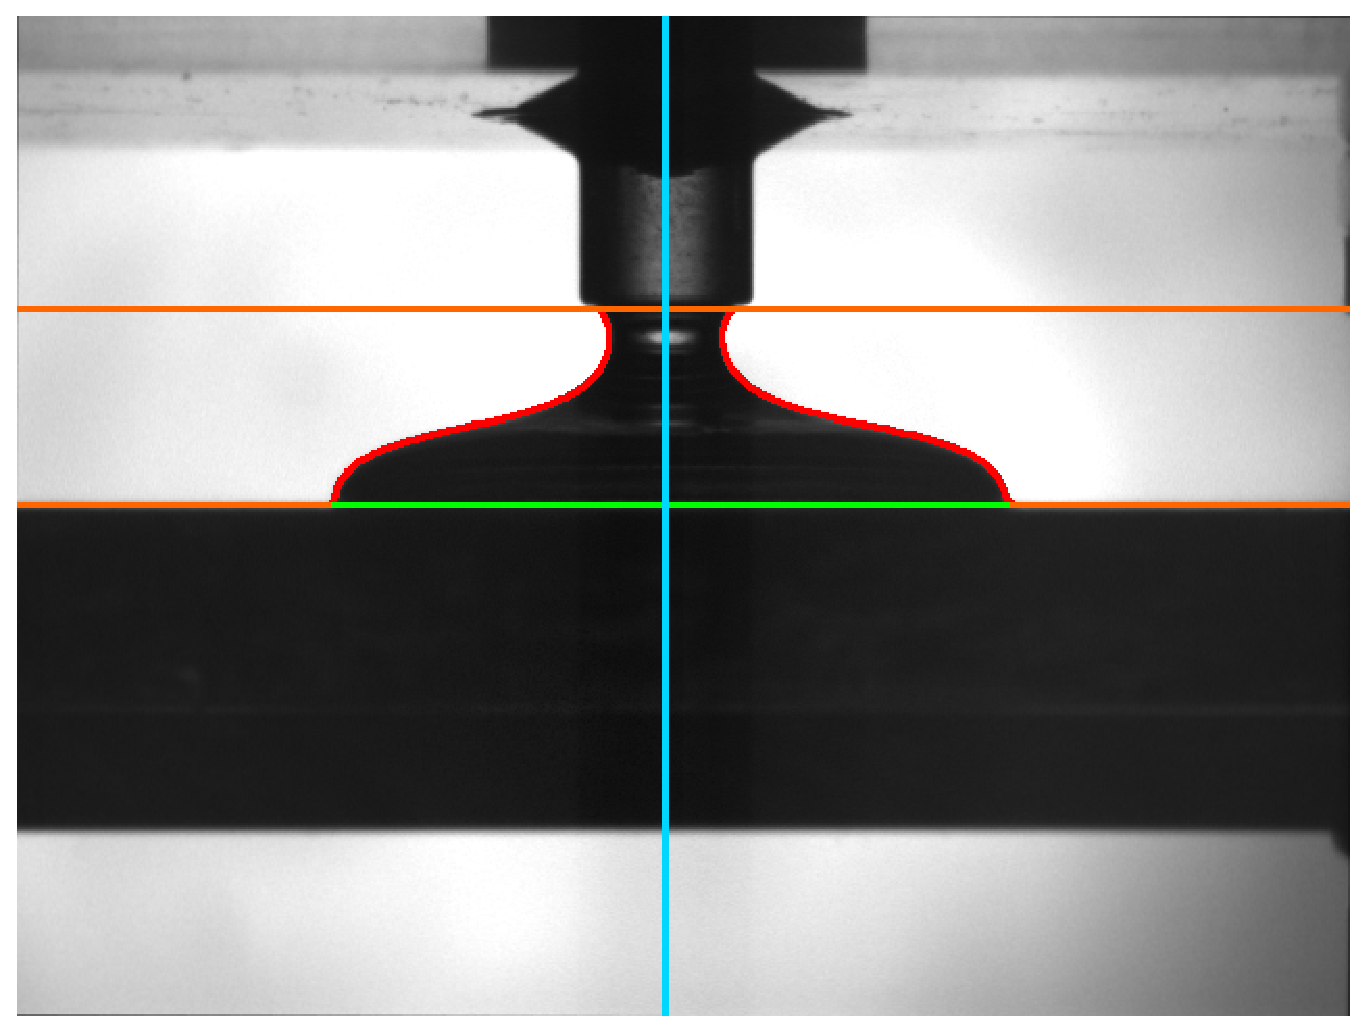
\includegraphics[trim={10px
       150px 10px
       75px},clip,width=0.4\textwidth]{figures/111014_glucose_syrup_thick_layer_8_0117_analysed.eps}}\addtocounter{subfigure}{-4}
 \\ \subfloat[\label{fig:111014_glucose_syrup_dry_substrate_3_0200_analysed}]{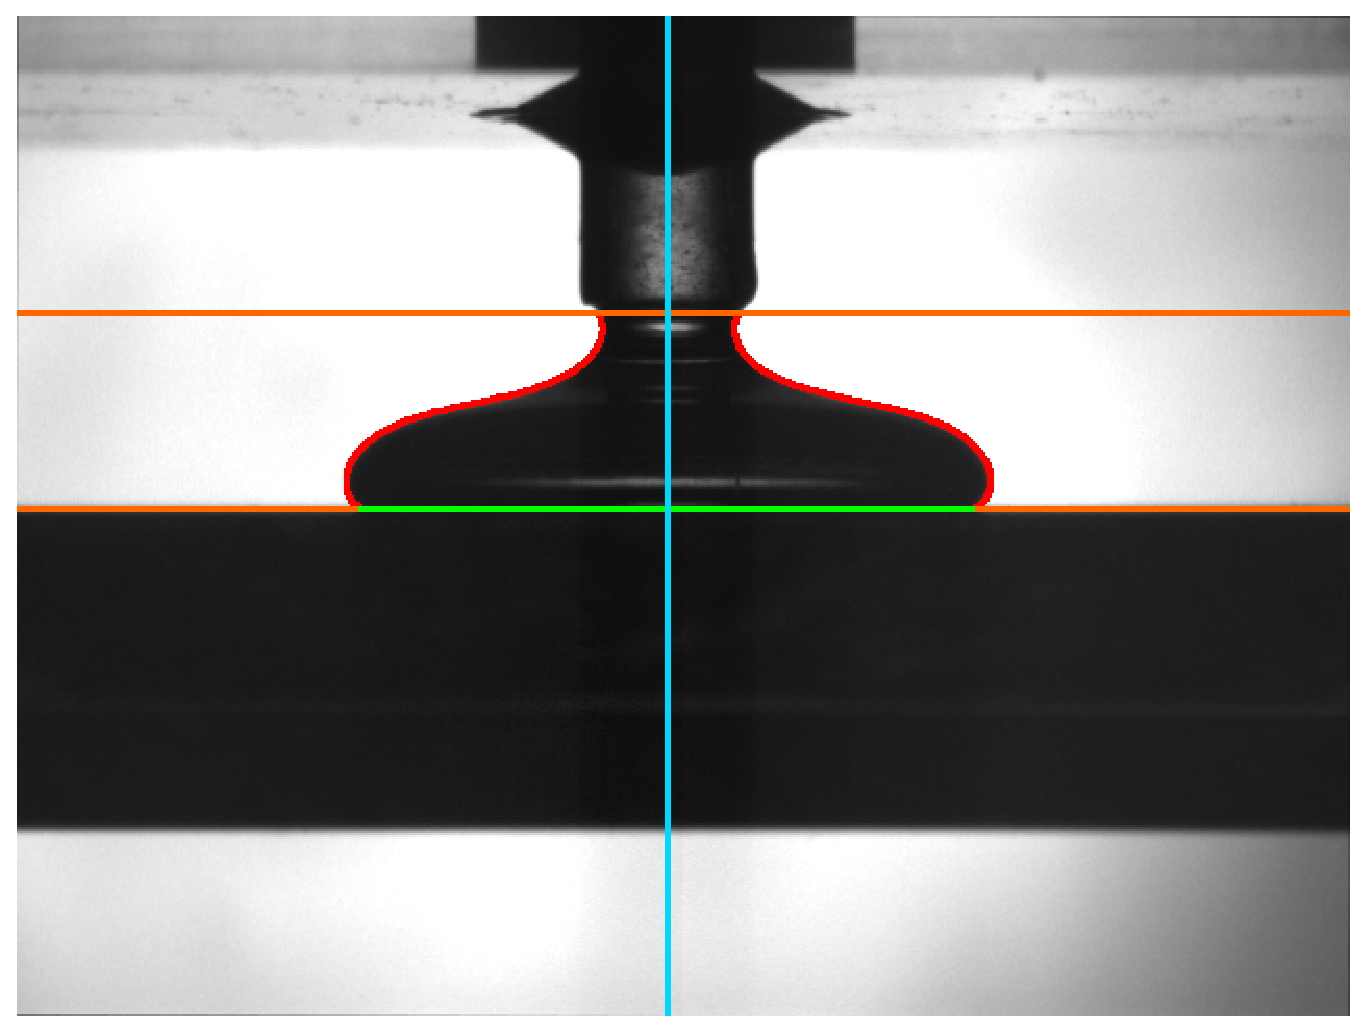
\includegraphics[trim={10px
       150px 10px
       75px},clip,width=0.4\textwidth]{figures/111014_glucose_syrup_dry_substrate_3_0200_analysed.eps}}\addtocounter{subfigure}{+3} \hspace{0.5cm}
 \subfloat[\label{fig:111014_glucose_syrup_thick_layer_8_0167_analysed}]{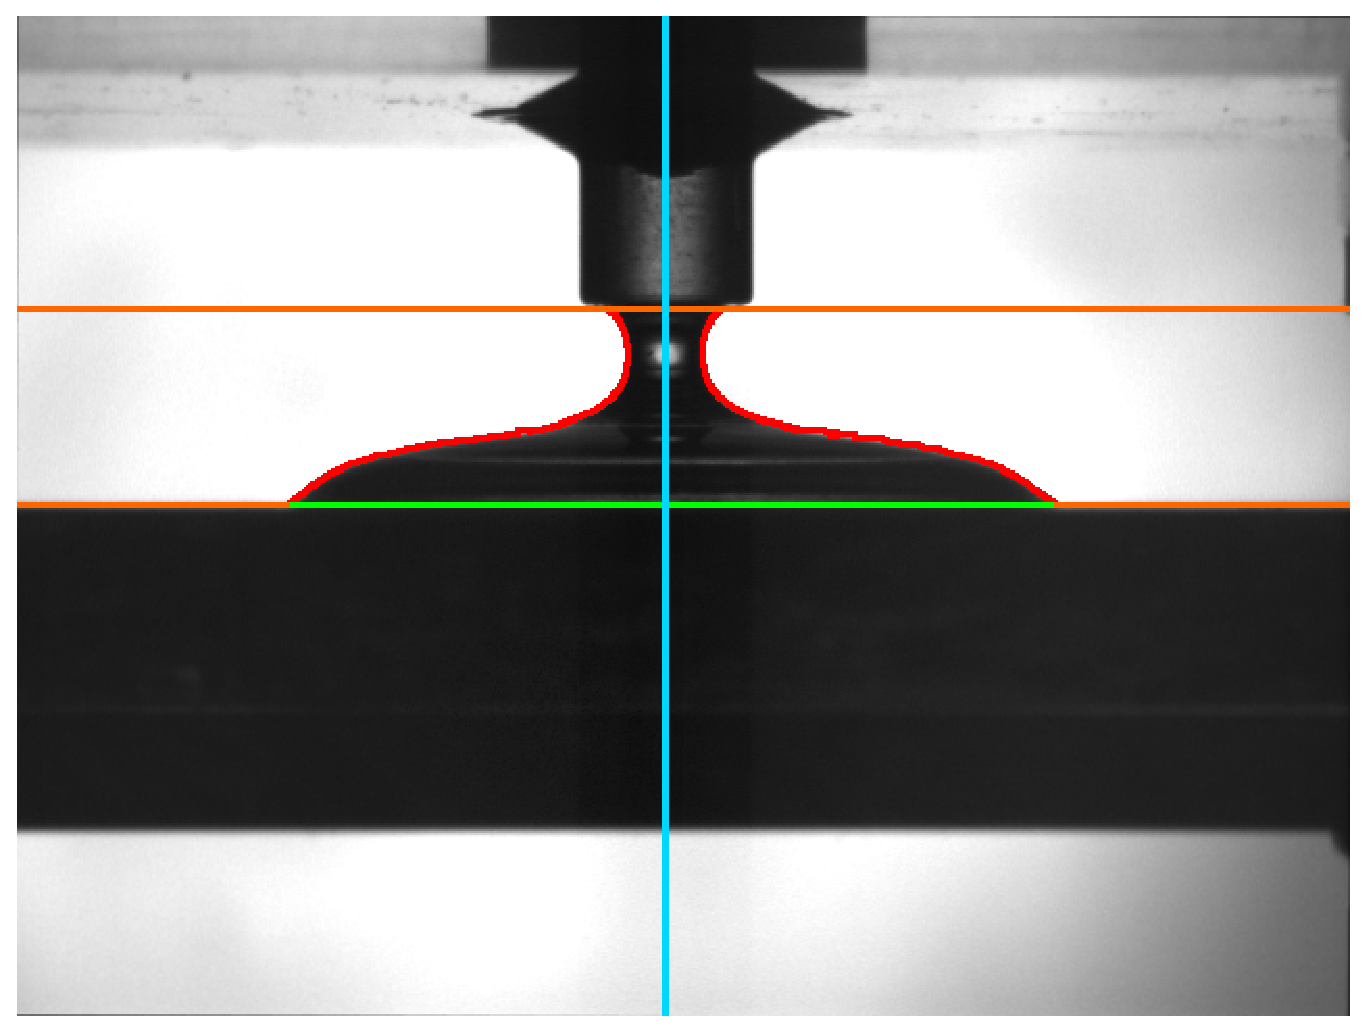
\includegraphics[trim={10px
       150px 10px
       75px},clip,width=0.4\textwidth]{figures/111014_glucose_syrup_thick_layer_8_0167_analysed.eps}}\addtocounter{subfigure}{-4}
 \\ \subfloat[\label{fig:111014_glucose_syrup_dry_substrate_3_0400_analysed}]{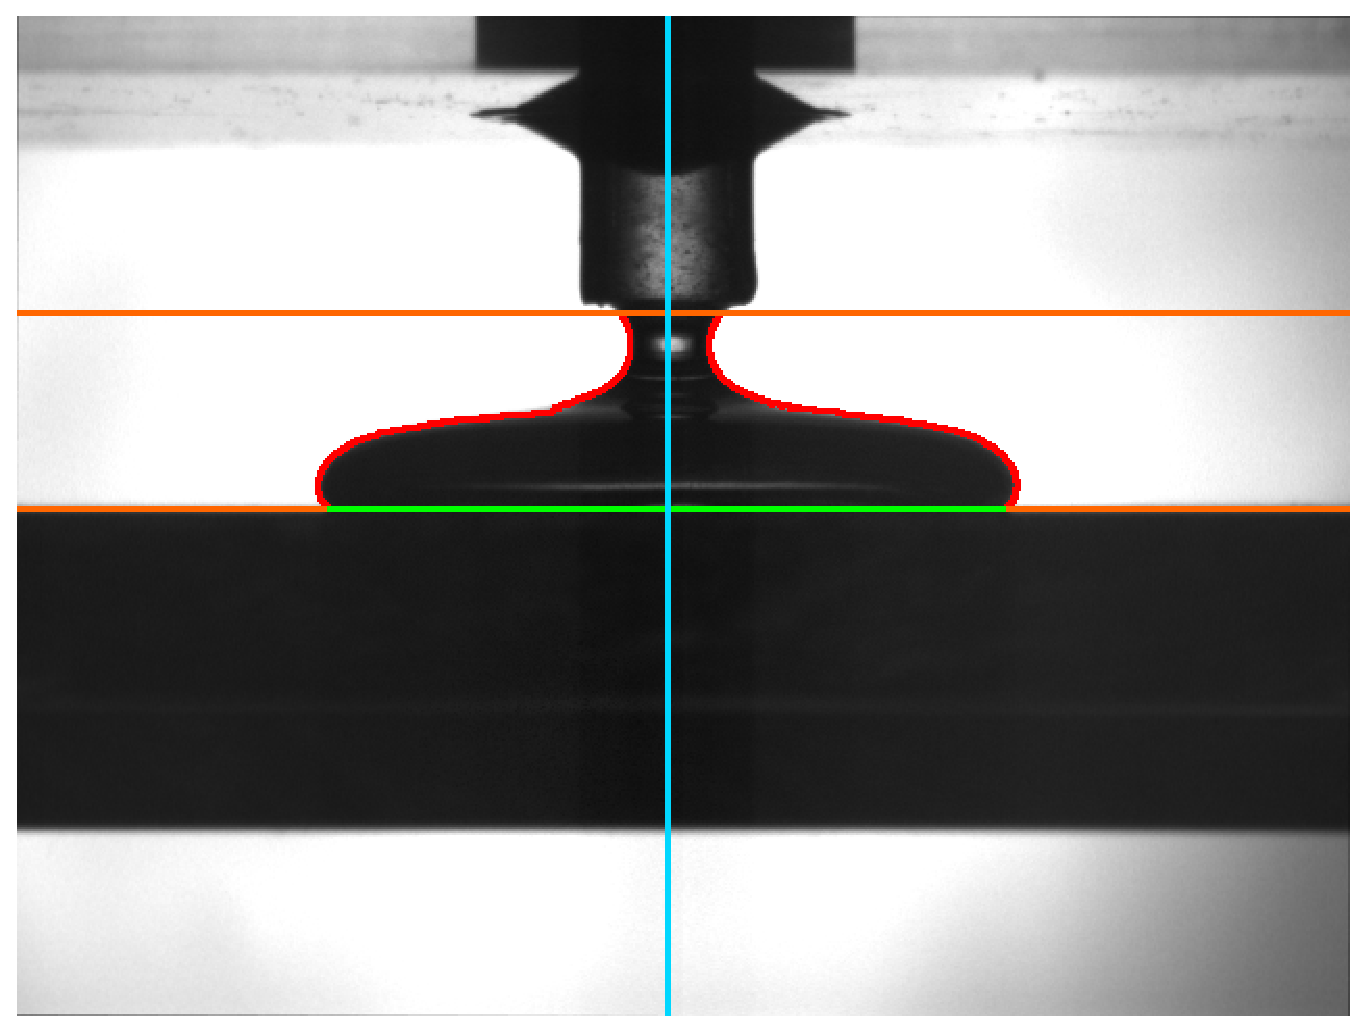
\includegraphics[trim={10px
       150px 10px
       75px},clip,width=0.4\textwidth]{figures/111014_glucose_syrup_dry_substrate_3_0400_analysed.eps}}\addtocounter{subfigure}{+3} \hspace{0.5cm}
 \subfloat[\label{fig:111014_glucose_syrup_thick_layer_8_0367_analysed}]{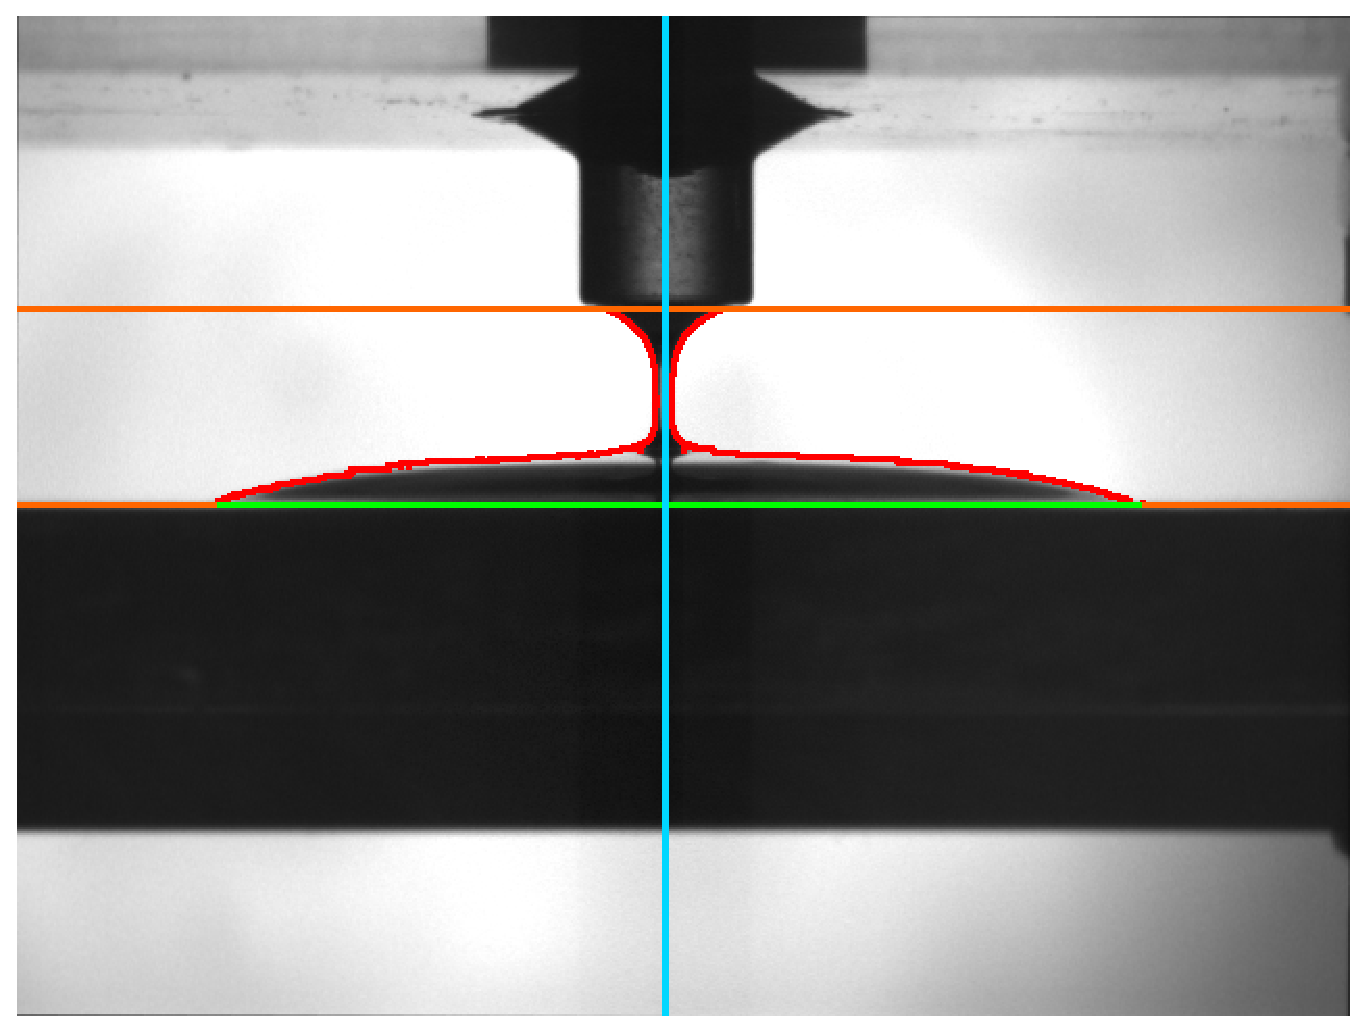
\includegraphics[trim={10px
       150px 10px
       75px},clip,width=0.4\textwidth]{figures/111014_glucose_syrup_thick_layer_8_0367_analysed.eps}}
  \caption{Side-view images of glucose syrup spreading on a dry
    substrate ( (a)-(d) ) and on a layer of
    the same fluid ( (e)-(h) ) at different times for a single experiment: (a)/(e)
    $t=0.0$ s, (b)/(f) $t=2.5$ s, (c)/(g) $t=5.0$ s, (d)/(h) $t=15.0$
    s. We show the processed images,
    highlighting the platform edge and nozzle end, centre line, bottom
    diameter and air-liquid interface.\label{fig:glucose_spreading}}
\end{figure}

Sequences of images showing the spreading of a drop
of glucose syrup on a dry substrate and on a layer of the same fluid are shown in Fig.
\ref{fig:glucose_spreading}. Figs. \ref{fig:glucose_spreading}(a) and (e)
show the initial drop configuration immediately after all the fluid 
has been ejected from the syringe. Figs. 
\ref{fig:glucose_spreading}(b-d) and (f-h) illustrate the subsequent,
approximately axisymmetric spreading of the drop. In both cases the spreading
rate decreases as the drop spreads out (note the non-uniform time
incremements between the different sub-figures). For the spreading
on a layer
the slope of the air-liquid interface near the advancing front 
becomes increasingly shallow, while the interface shape near the
advancing front remains largely unchanged during the spreading on a dry substrate. The radius of the thread of fluid that connects
the drop to the nozzle decreases rapidly and the thread ultimately 
pinches off (not shown here). The detached lower half of the thread 
then collapses onto surface of the drop where it tended to create 
additional reflections which made the subsequent image processing 
difficult. However, the pinch-off of the thread had little effect on the 
overall spreading dynamics. We refer to \S \ref{sec:influence_layer_thickness} for a more detailed
assessment of the pinch-off.

%\begin{figure}[!ht]
%\centering
%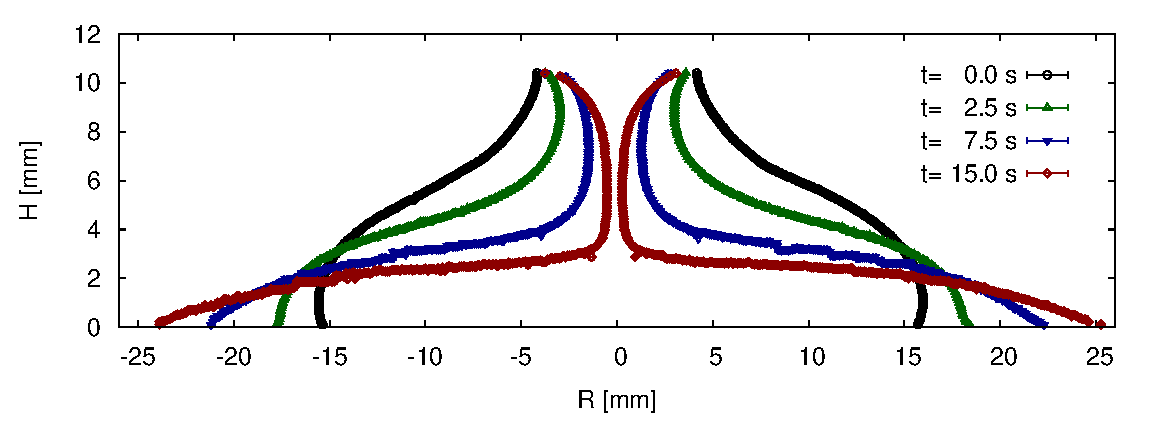
\includegraphics[width=0.9\textwidth]{figures/glucose_thick_layer_8_fs_dim.eps}
%\caption{Free surface extracted for a single experiment at different
%  times $t$.}
%\label{fig:glucose_thick_layer_8_fs_dim}
%\end{figure}


\begin{figure}[!ht]
\centering
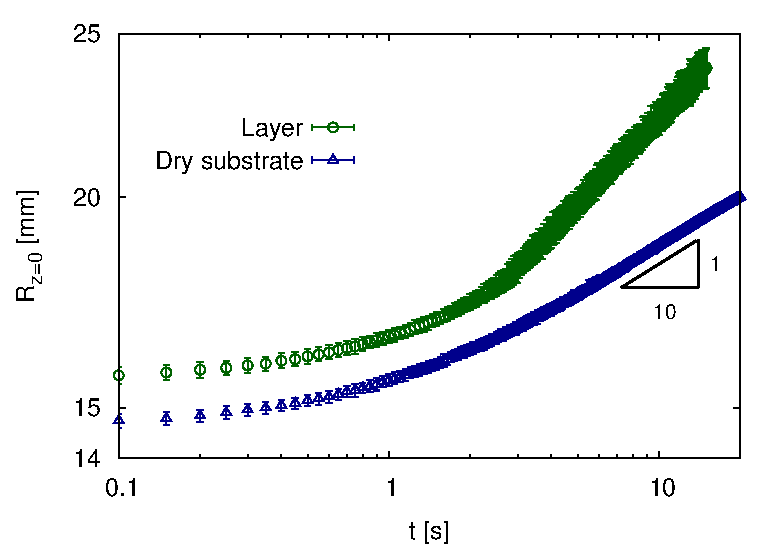
\includegraphics[width=0.6\textwidth]{figures/radius_vs_time_comp_layer_dry.eps}
\caption{Mean radius evolution and error bars across five experiments each, for
  spreading on a layer of fluid (green circles) and on a dry substrate
  (blue triangles), on a log-log
  scale. }
\label{fig:diam_vs_time_comp_layer_dry}
\end{figure}


Fig. \ref{fig:diam_vs_time_comp_layer_dry} shows the time-evolution
of the drop radius $R_{z=0}$ (measured at the upper surface
of the substrate; green circles) on a log-log scale and
contrasts it with the evolution for spreading of an equivalent drop 
on a dry substrate (blue triangles). The initial evolution 
of the radii up to a time of approximately 2 s is very similar for the two 
cases, suggesting that the initial (short-time) spreading dynamics are
independent of the substrate on which the drop spreads.
Beyond this time the drop deposited on the dry substrate spreads
significantly more slowly than that deposited on the fluid layer.
For the drop on the dry substrate, the moving contact line can be
observed throughout the evolution since it is not obscured by the
trough. The figure shows that the contact line motion follows
the power-law behaviour $R \sim t^{1/10}$ predicted by scaling
arguments based on a balance between capillary and viscous forces
\cite{tanner1979spreading}, and also observed in previous experimental
work by Cazabat and Cohen Stuart\cite{cazabat1986dynamics}.
The scaling arguments for this power-law behaviour are based
on the assumption of small drops with a radius much less
than the capillary length, $R \ll l_c$.
In our experiments, however, $R \gg l_c$ with $l_c \approx 2$ mm and
therefore this small drop assumption does not hold.
Instead for large drops, where surface tension becomes negligible, a power-law behaviour with $n=1/8$ based on a
balance between gravitational and viscous forces was found
theoretically \cite{lopez1976spreading} and observed experimentally
\cite{cazabat1986dynamics,huppert1982propagation}.
However, our
experimental exponent differs from the $n=1/8$ exponent obtained for
such axisymmetric gravity currents.
This could indicate that the gravity dominated spreading is not yet
realised and the spreading shown in Fig.
\ref{fig:diam_vs_time_comp_layer_dry} only captures the short-term
behaviour, which is dominated by capillary forces.
This is consistent with the experimental observations by Cazabat and
Cohen Stuart\cite{cazabat1986dynamics}, who reported short-term (1 min) capillarity
driven spreading followed by a transition to gravity driven spreading.


\section{Computations}

\subsection{Computational model}

\subsubsection{Governing equations}

We model the glucose syrup as an incompressible Newtonian fluid
and scale the velocities on the characteristic settling velocity of a sessile drop
under gravity, $\mathcal{U}=(\rho g \mathcal{L}^2) / \mu$, and all
lengthscales on the outer radius of the nozzle outlet, $R_{\sym{outlet}}^*$. 
The flow is then
governed by the non-dimensional Navier-Stokes equations

\begin{equation}
 \sym{Re} \Bigg( \sym{St} \pder[\vect{u}]{t} + (\vect{u} \cdot \nabla)
 \vect{u} \Bigg) = - \nabla p + \frac{\sym{Re}}{\sym{Fr}} \: \vect{G}
 + \nabla^2 \vect{u},
 \label{eqn:ns_eqn_momentum_nondim}
\end{equation}
and
\begin{equation}
 \nabla \cdot \vect{u} = 0.
 \label{eqn:ns_eqn_continuity_nondim}
\end{equation}

%\begin{figure}[!ht]
%\centering
%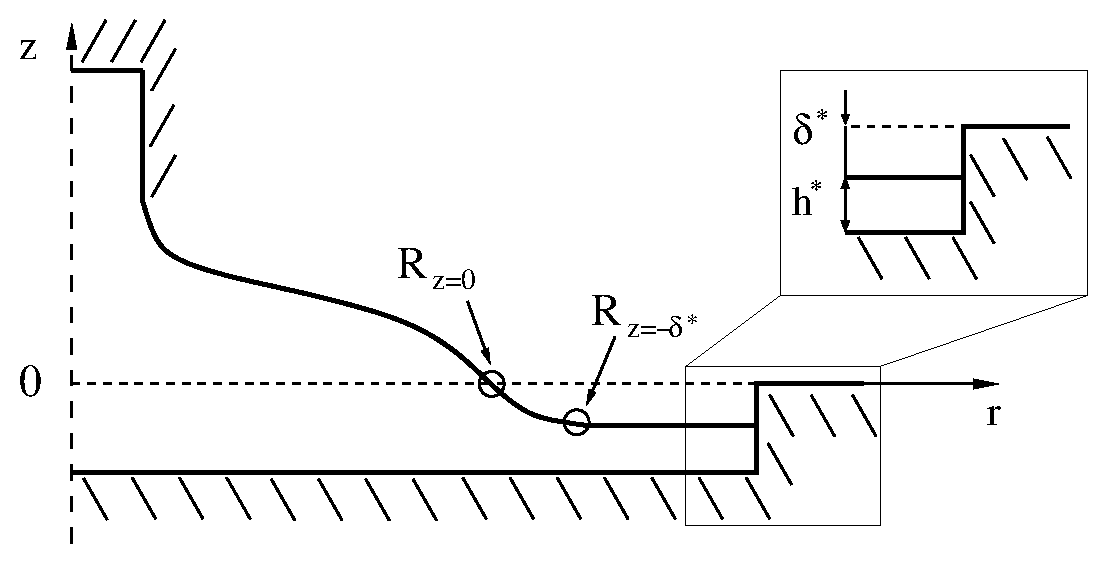
\includegraphics[width=0.6\textwidth]{figures/axisym_drop_nozzle_gap_computation_updated.eps}
%\caption{Schematic diagram of a model in cylindrical polar coordinates
%  of the experiment investigating the spreading of a drop on a layer
%  of the same fluid, where $R_{z=0}(t)$ is the
%  experimentally visible drop radius and $R_{z=-\delta^*}(t)$ is the
%  radius of the propagating front.}
%\label{fig:axisym_drop_nozzle}
%\end{figure}

We solve equations (\ref{eqn:ns_eqn_momentum_nondim}) and (\ref{eqn:ns_eqn_continuity_nondim}) in cylindrical polar coordinates, with the
assumption that there is no variation in the azimuthal direction
($\partial / \partial \phi = 0$), so that it becomes an axisymmetric
flow problem in the two spatial dimensions $\vect{x}=\{r,z\}$.
Moreover, we assume that there is no swirl, $u_{\phi}=0$, so that the
velocity field is $\vect{u}=\{u_r,u_z\}$.  Also, the gravitational
acceleration is only acting in the axial direction, $G_z = -1$ and
$G_i=0, i = \{ r,\phi \}$.  On the solid walls we apply no-slip,
$\vect{u} = 0$, and the centre line of the drop, at $r=0$, is a symmetry
boundary with $u_r = 0$ and $\partial u_z / \partial r = 0$.
At the air-liquid interface we apply the dynamic and kinematic
boundary condition,
 $\vect{\sigma} \cdot \vect{n} = 1/\sym{Ca} \; \kappa \; \vect{n}
-p_{\sym{ext}} \; \vect{n}$ and
 $( \vect{u} - \sym{St} \: \partial \vect{R}_{\sym{fs}} / \partial t ) \cdot \vect{n} = 0$, respectively,
where $\vect{n}$ is the outer unit normal to the interface $\vect{R}_{\sym{fs}}$,
pointing out of the liquid. 


In order to validate the computations against the experimentally
observed flow, we numerically model the single spreading experiment
on a layer as presented in section \ref{sec:exp_results}.
The other experiments for the spreading on a layer are qualitatively
similar and are therefore not specifically discussed here.  The initial
shape of the free surface in the computation is constructed based on
the free surface location determined during the experimental analysis.
However, the computation is limited to one side of the free surface,
because axisymmetric flow is assumed and we arbitrarily chose the
right-hand surface of the drop.  As discussed in section
\ref{sec:creating_layer} we found experimentally that there is a gap
$\delta^*$ between the fluid layer and platform edge which means that
part of the drop surface is invisible in the experiment.  The size of this gap was
difficult to determine accurately and was therefore estimated at
$\delta^*=1.15$ mm, resulting in an estimated uniform fluid layer
thickness of $h^*=0.85$ mm.  However, through numerical experiments we
found that the actual layer thickness was $h^*=1.25$ mm and the
results for the estimated and computationally re-constructed layer
thickness are compared in section \ref{sec:comp_spreading_on_layer}.
For the flow simulation we re-constructed the experimentally invisible
part of the free surface by fitting a spline through the points on the
uniform fluid layer and the visible part of the surface.

\subsubsection{Non-dimensional parameters}

The non-dimensional
parameters that enter the Navier-Stokes equations directly are given
by

\begin{gather}
 \sym{Re} = \frac{\rho \: \mathcal{U L}}{\mu} = \frac{\rho^2 \: g \:
   R_{\sym{outlet}}^{*3}}{\mu^2}, \qquad \sym{St} =
 \frac{\mathcal{L}}{\mathcal{U} \mathcal{T}} = 1, \qquad \sym{Fr} =
 \frac{\mathcal{U}^2}{g \: \mathcal{L}} = \frac{\rho^2 \: g \:
   R_{\sym{outlet}}^{*3}}{\mu^2} = \sym{Re}, \nonumber \\[0.75cm]
 \sym{Ca} = \frac{\mu \: \mathcal{U}}{\sigma} = \frac{\rho \: g \:
   R_{\sym{outlet}}^{*2}}{\sigma},
 \label{eqn:nondim_numbers}
\end{gather}
where we chose the
intrinsic timescale $\mathcal{T}=\mathcal{L}/\mathcal{U}$ as the reference timescale for the setup, resulting in a unit Strouhal number.
For our choice of non-dimensionalisation, $\sym{Ca}$ is independent
of the viscosity and $\sym{Fr}=\sym{Re}$, so that $\sym{Re}/\sym{Fr} =
1$.
The length scale of the problem is the outer radius of the nozzle
outlet $\mathcal{L}=R_{\sym{outlet}}^*=4.61$ mm.
The characteristic velocity and time scales are $\mathcal{U}=6.563
\times 10^{-3}$ m/s and $\mathcal{T}=7.025 \times 10^{-1}$ s,
respectively.
The gravitational acceleration is $g=9.81$ m/s$^2$.
The material properties are taken from \S \ref{sec:experimental_setup}
at a temperature of 20.3 $^{\circ}$C, which was the temperature
recorded for the experiment.
Hence, the fluid density is $\rho=1372.8$ kg/m$^3$ and its viscosity $\mu=43.61$
Pa.s.
The surface tension of the glucose syrup was taken from the 
literature \cite{montanez2013influence} as $\sigma=55.0 \pm 0.6 \times
10^{-3}$~N/m.
The length of the syringe nozzle is $L_{\sym{nozzle}}^*=10.0$ mm.
The radius of the trough is $R_{\sym{trough}}^*=30.25$ mm and the
distance between the fluid layer and the upper edge of the substrate
is $\delta^*=0.75$ mm.
We vary the layer thickness in our simulations in the range $h^*=0.005
- 12.5$ mm, while keeping $\delta^*$ fixed (unless stated otherwise).
The values of the resulting non-dimensional numbers are

\begin{equation}
 \sym{Re} = \sym{Fr} = 9.523 \times 10^{-4}, \qquad \sym{St}=1, \qquad
 \sym{Ca}=5.204,
\end{equation}
and the geometric values are

\begin{equation}
 h = 1.085 \times 10^{-3} - 2.711 \times 10^{0}, \quad \delta=0.16269, \quad R_{\sym{trough}}=6.562, \quad
 L_{\sym{outlet}}=2.169.
\end{equation}

\subsubsection{Discretisation in FEM}

We discretised the fluid domain and domain boundary using the
finite element method (FEM) as implemented in \texttt{oomph-lib}
\cite{HeilHazelOomph2006}.  Flow problems involving free surfaces are
conveniently represented using unstructured meshes with triangular
elements, because it is challenging to represent complex interface
shapes using structured meshes with a set of rectangular elements.
Therefore, we used triangular elements in an axisymmetric coordinate
systems and we generated the unstructured meshes using
\texttt{Triangle} \cite{shewchuk96b}.  Specifically, we used
six-noded, triangular Taylor-Hood \cite{taylor1973numerical} elements
($P_2 P_1$) with a maximum element area of 0.05.  The Taylor-Hood
elements satisfy the Lady\u{z}enskaja-Babu\u{s}ka-Brezzi (LBB)
condition \cite{sani2000incompressible}, which means that they do not
feature any spurious pressure modes.  Moreover, the solution obtained
with these elements is guaranteed to converge at the optimal,
quadratic convergence rate under mesh refinement
\cite{donea2003finite}.  In the free-surface problem that we modelled,
the domain is moving and it is discretised using an unstructured mesh
which is fitted to the fluid domain.  Hence, the mesh is deforming in
response to the motion of the fluid, which we realised by using the
Arbitrary Lagrangian Eulerian (ALE) method \cite{donea1982arbitrary}.
Specifically, the change of the mesh shape is driven by the motion of
the free surface.  Additional unknowns are introduced, because the
location of the free surface $\vect{R}_{\sym{fs}}$ is unknown and has
to be determined during the solution process.  The additional
equations that need to be solved to obtain $\vect{R}_{\sym{fs}}$ arise
from the kinematic boundary condition.  At every timestep the location
of the free surface is determined and the positions of the nodes in
the mesh are updated accordingly employing a pseudo-solid mesh
approach.  The pseudo-solid node-update procedure treats the mesh as
an elastic body, which deforms, and at every timestep a solid
mechanics problem needs to be solved simultaneously with the fluids
problem to compute the unknown nodal positions.  The position of the
free surface is imposed by artificial pressures acting normal to the
interface, which have the function of Lagrange multipliers and are
obtained through the solution of the kinematic boundary condition.
Although this approach is computationally expensive as it introduces
two additional unknowns at each node and a solid mechanics problem has
to be solved at each timestep, it enables the simulation of flows with
complex free surface shapes, which is required for our problem.  In
the process of timestepping, the elements in the mesh become
increasingly distorted, because the node positions are constantly
updated.  Therefore we re-generated the mesh after every two time
steps based on the current position of the domain boundaries and the
current solution is projected across onto the new mesh.  We performed
time-dependent simulations and used a second-order accurate Backward
Differentiation Formula (BDF2) scheme \cite{sani2000incompressible}
for the temporal discretisation.  In order to enable direct comparison
with the experiment, the flow was simulated for the duration of the
experiment, $t^*_{\sym{exp}}=15$ s.  The time step in the temporal
discretisation was chosen as the time difference between successive
frames in the experiment, $\Delta t^*_{\sym{exp}} = 0.05$ s.  We
performed mesh independence studies, which showed that the chosen
spatial and temporal discretisation accurately resolve the problem.

\subsection{Computational results}

\subsubsection{Spreading on a layer}
\label{sec:comp_spreading_on_layer}

\begin{figure}[!ht]
\centering
\begin{postscript}
 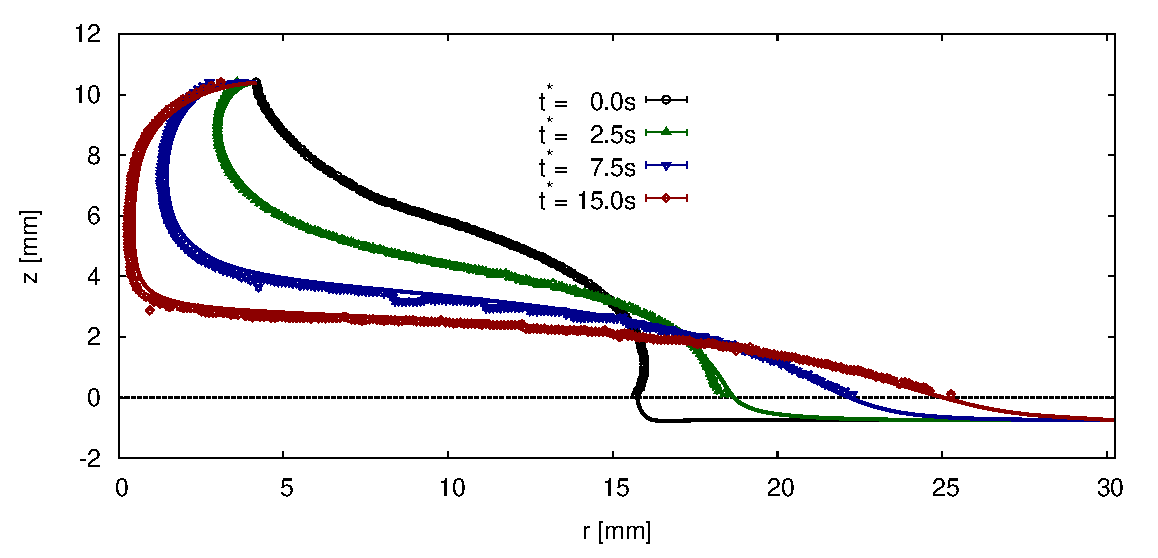
\includegraphics[width=0.9\textwidth]{figures/glucose_thick_layer_8_fs_dim_gap_0.75mm.eps}
 \rput(-2.0,4.5){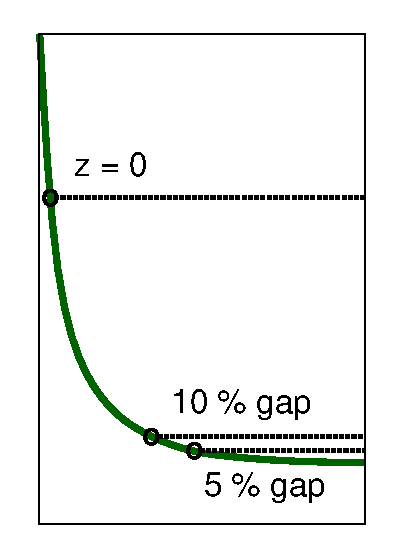
\includegraphics[width=0.19\textwidth]{figures/glucose_thick_layer_8_fs_dim_gap_0.75mm_meas_pt.eps}}
\end{postscript}
\caption{Free surface at different times for a layer thickness of
  $h^*=1.25$ mm compared against the experiment. Points represent the
  free surface shape in the experiment; lines represent the computed
  free surface. Inset shows different measurement points for the drop
  radius.}
\label{fig:glucose_thick_layer_8_fs_dim_gap_0.75mm}
\end{figure}

The computed shape of the free surface of the spreading drop,
$\vect{R}^*_{\sym{fs}}(t)$, at different dimensional times $t^*$ is
compared against the experimentally determined shape in Fig.
\ref{fig:glucose_thick_layer_8_fs_dim_gap_0.75mm}, where the error
bars represent the pixelation error of the image analysis.  There is
excellent agreement between the computations and experiment and the
computations provide additional insight into the profile for $z<0$.
As the drop spreads out its height reduces and the fluid thread
between the bulk of the drop and the residual fluid in the nozzle
outlet narrows.  The radius of this thread decreases, resulting
eventually in pinch-off due to the Plateau-Rayleigh instability.
However, the computation was stopped before the pinch-off.  Moreover,
there is a significant change of the free surface shape in the region
between the drop and the fluid layer.  Initially, the curvature in
this region is high, but as the drop spreads the interface is pushed
out and the curvature decreases until the free surface forms a wedge
which advances.

\begin{figure}[!ht]
\centering
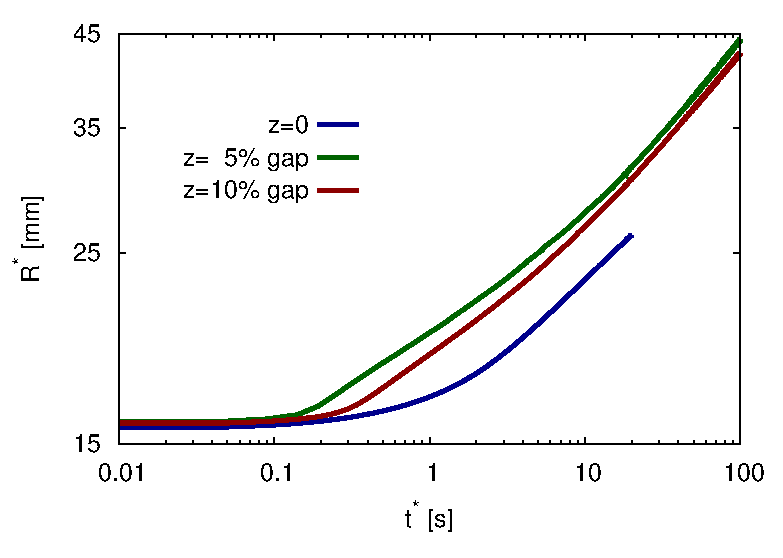
\includegraphics[width=0.6\textwidth]{figures/radius_vs_time_measure_pos_dim.eps}
\caption{Temporal evolution of the drop radius at different
  measurement points on a log-log scale.}
\label{fig:glucose_thick_layer_8_radius_vs_time_non_dim}
\end{figure}

The evolution of the drop radius is shown in Fig.
\ref{fig:glucose_thick_layer_8_radius_vs_time_non_dim} on a log-log
scale at different measurement points.  The radius is determined at
the level of the platform edge, as in the experiment, and at the
points where the gap is 5\% and 10\% filled (see Fig.
\ref{fig:glucose_thick_layer_8_fs_dim_gap_0.75mm}).  The radius
evolution at $z=0$ is not plotted over the entire range, because at
larger times the drop height decreases to $H^* < 0$ and hence no
radius at $z=0$ can be determined. The drop spreading based on the radius determined at a 5\%
and 10\% filled gap, respectively, is similar and the spreading law is
identical for $t^*>20$ s.  The spreading based on the radius at $z=0$
is significantly different and does not represent the actual dynamics.

\begin{figure}[!ht]
\centering
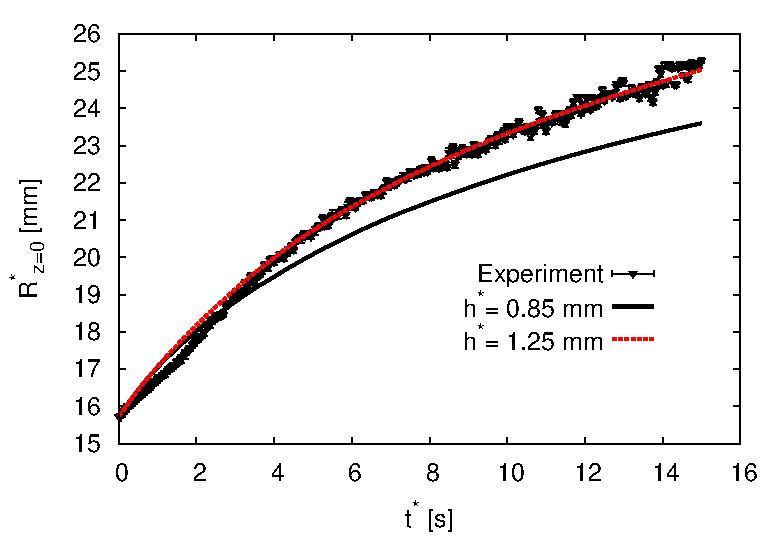
\includegraphics[width=0.6\textwidth]{figures/glucose_thick_layer_8_radius_vs_time_vary_layer.eps}
\caption{Evolution of $R^*_{z=0}$ over time for varying
  layer thicknesses $h^*$, compared against the experimentally
  determined radius.}
\label{fig:glucose_thick_layer_8_radius_vs_time_vary_layer}
\end{figure}

The radius evolution from the experiments at $z=0$ is compared against
the computed one in Fig.
\ref{fig:glucose_thick_layer_8_radius_vs_time_vary_layer}, for both
the experimentally estimated layer thickness of $h^*=0.85$ mm (and $\delta^*=1.15$ mm) and the
computationally re-constructed layer thickness of $h^*=1.25$ mm, which
we determined to fit the experimental radius evolution.  This figure
indicates that the layer thickness has strong influence on the drop
spreading, which motivated further numerical experiments.

\subsubsection{Influence of layer thickness\label{sec:influence_layer_thickness}}

\begin{table}[!ht]
 \centering
 \begin{tabular}{l | >{\centering\arraybackslash}m{3.5cm} | >{\centering\arraybackslash}m{3.5cm} | >{\centering\arraybackslash}m{3.5cm}}
   & \multicolumn{3}{>{\centering\arraybackslash}m{10.5cm}}{$h^*$ in
     mm} \\ \cline{2-4} $t$ & 0.0125 & 1.25 & 12.5 \\ \hline 0 &
  \begin{postscript}
   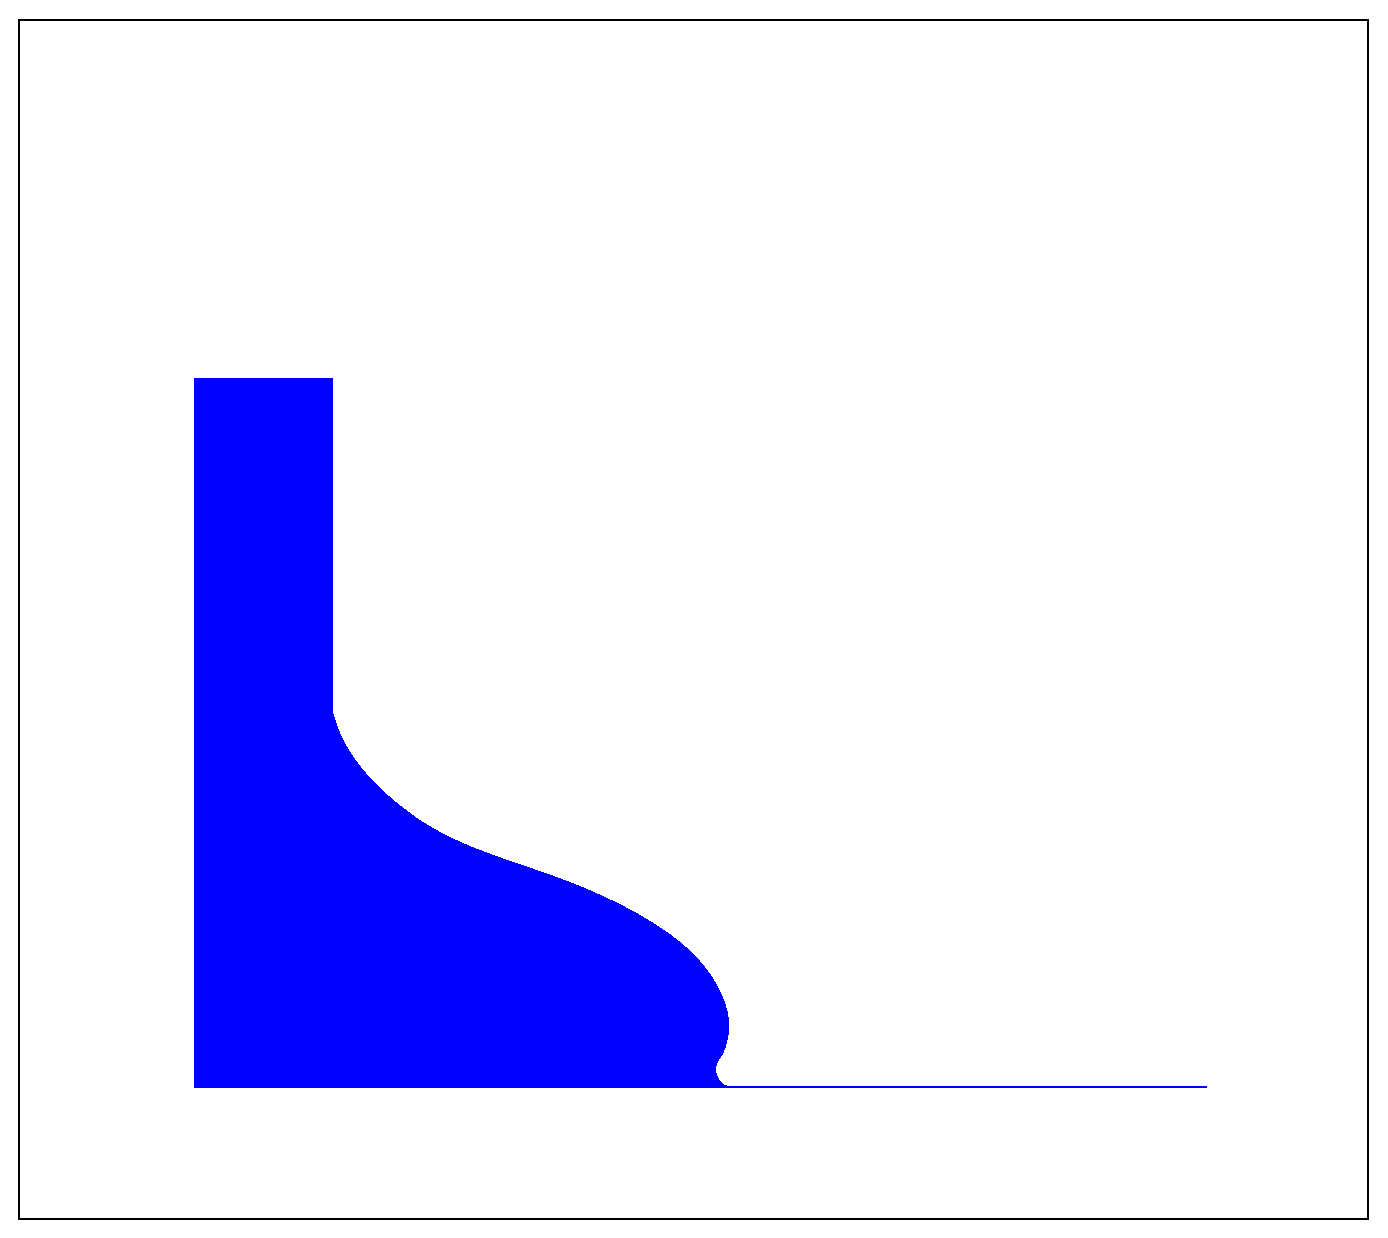
\includegraphics[trim={45px 35px 35px
       35px},clip,width=3.2cm]{figures/glucose_layer_0_0125mm_0_t_0.eps}
   \rput(-1.0,1.7){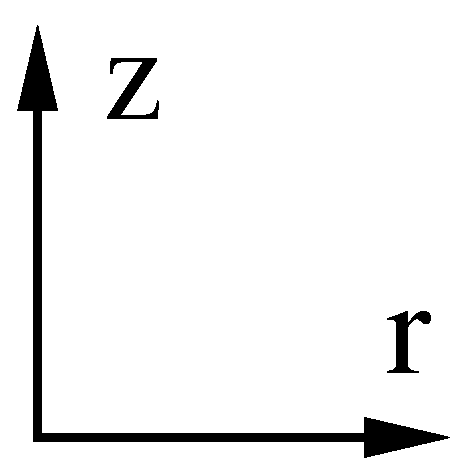
\includegraphics[width=1.25cm]{figures/axisym_coord.eps}}
  \end{postscript}
   & 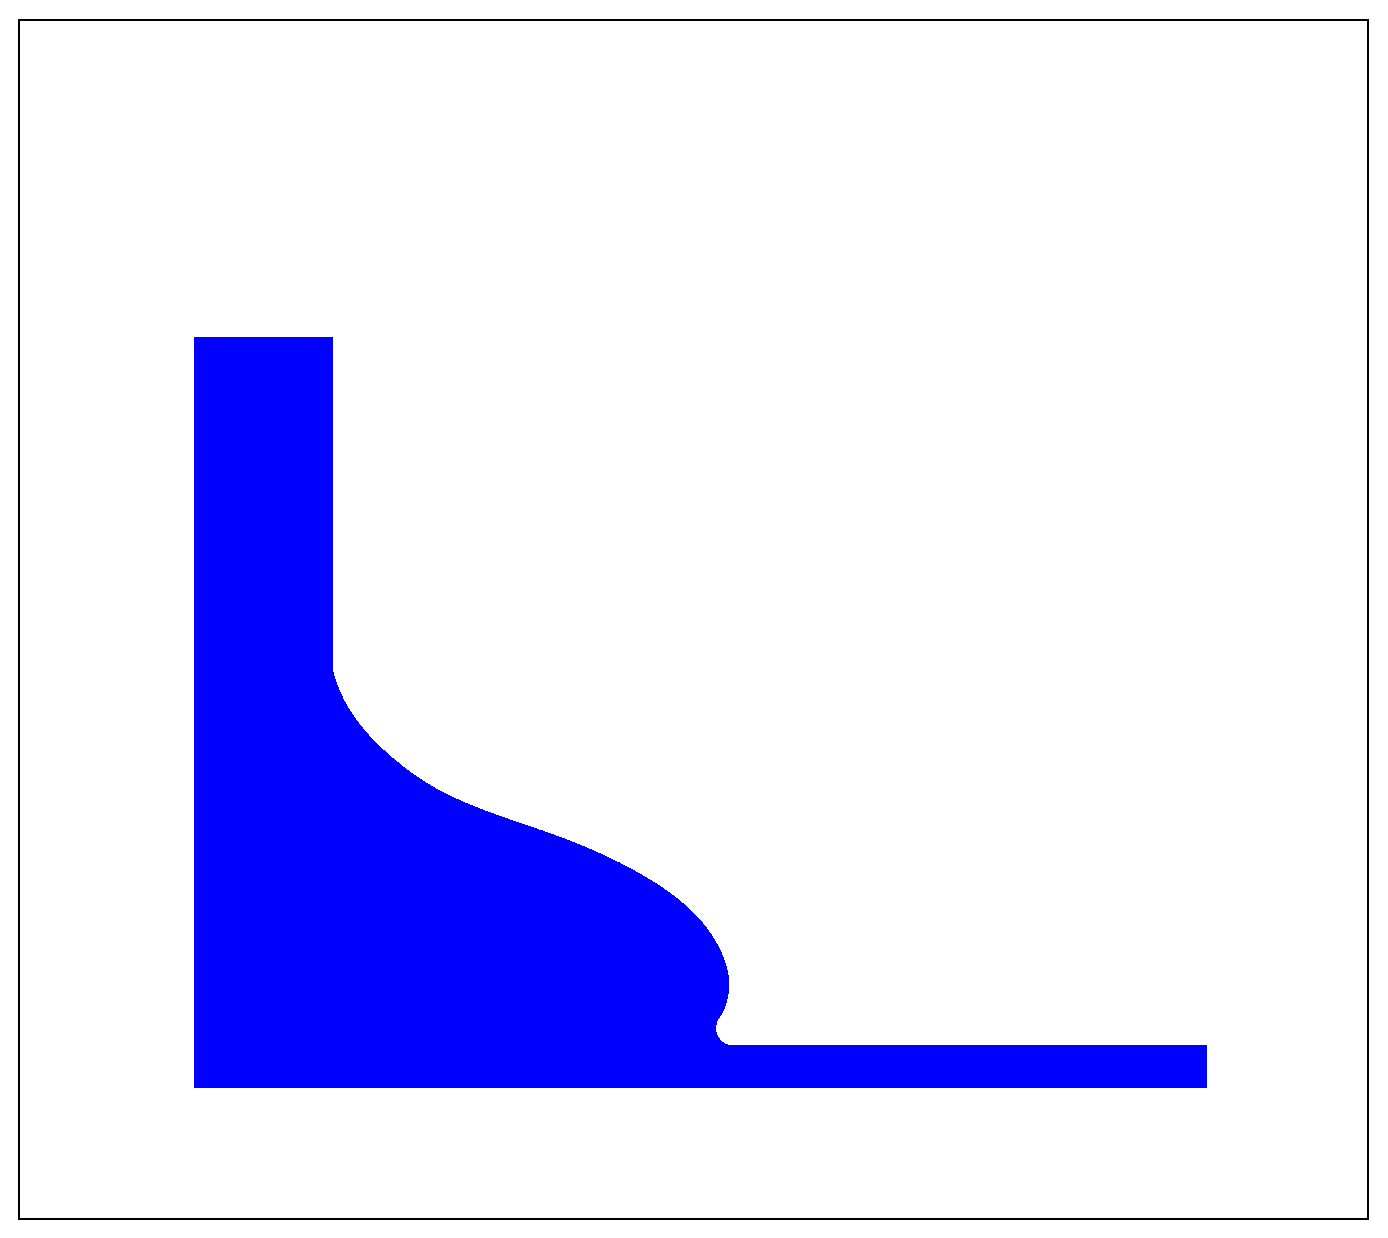
\includegraphics[trim={45px 35px 35px
      35px},clip,width=3.2cm]{figures/glucose_layer_1_25mm_0_t_0.eps}
  & 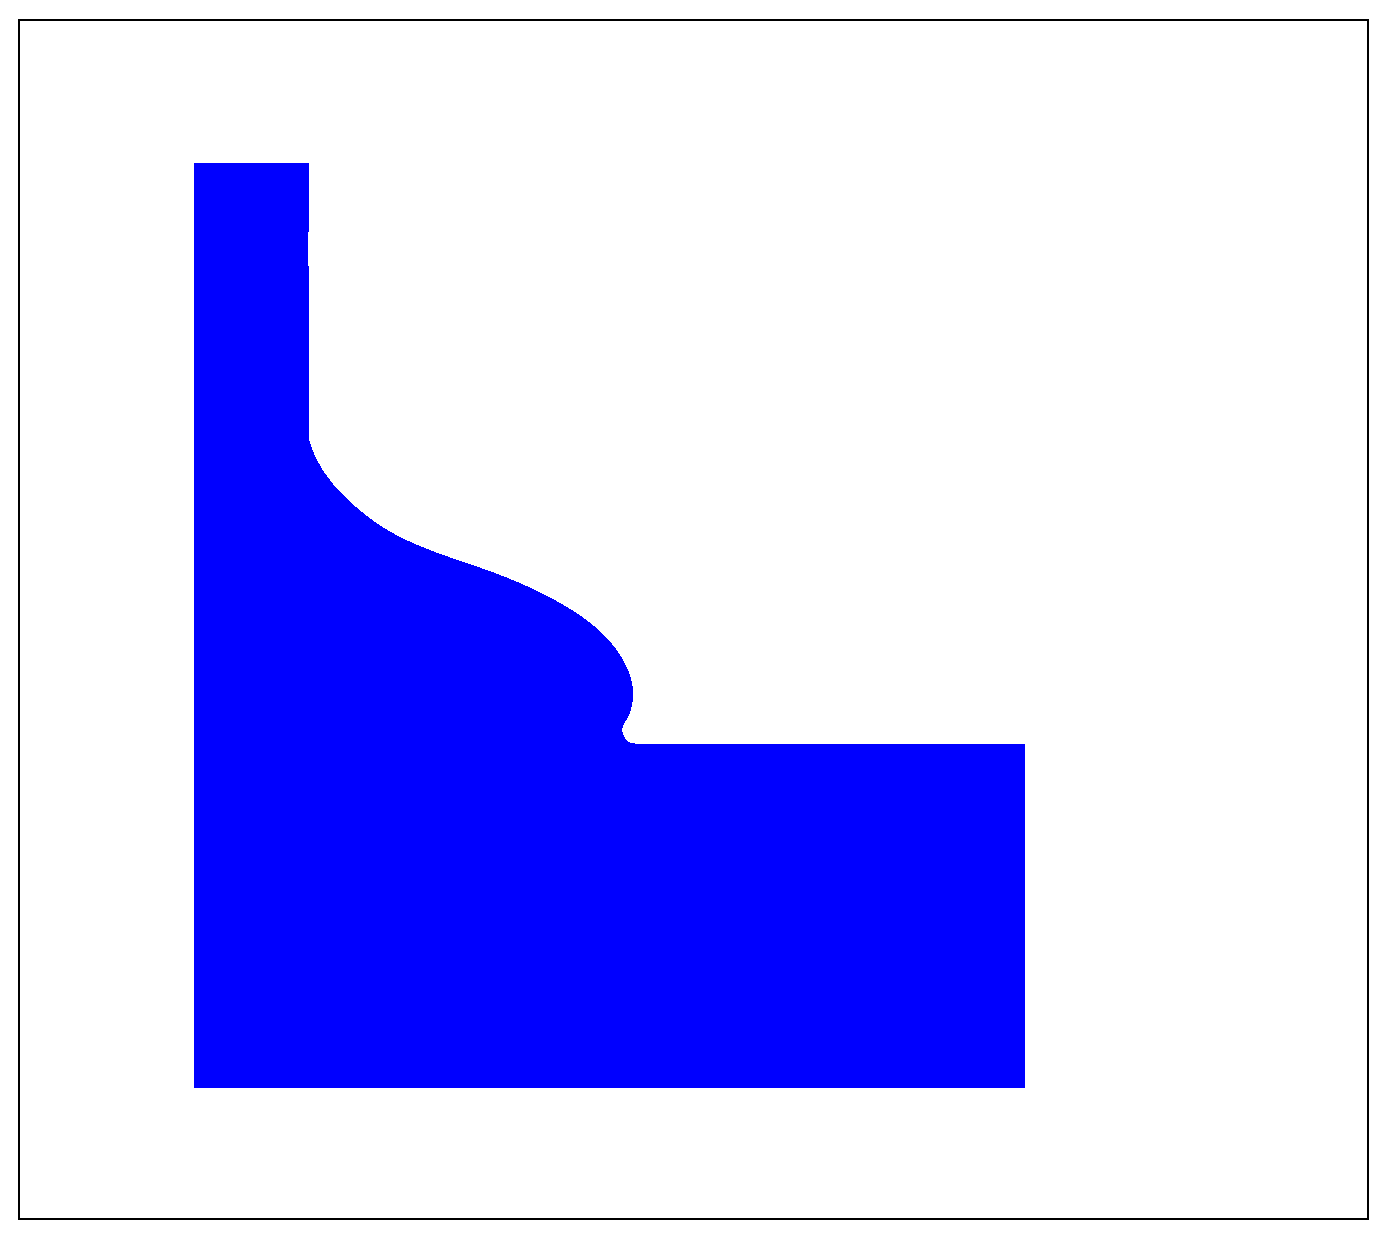
\includegraphics[trim={45px 35px 35px
      35px},clip,width=3.2cm]{figures/glucose_layer_12_5mm_0_t_0.eps}
  \\ \hline 2 &
  \begin{postscript}
   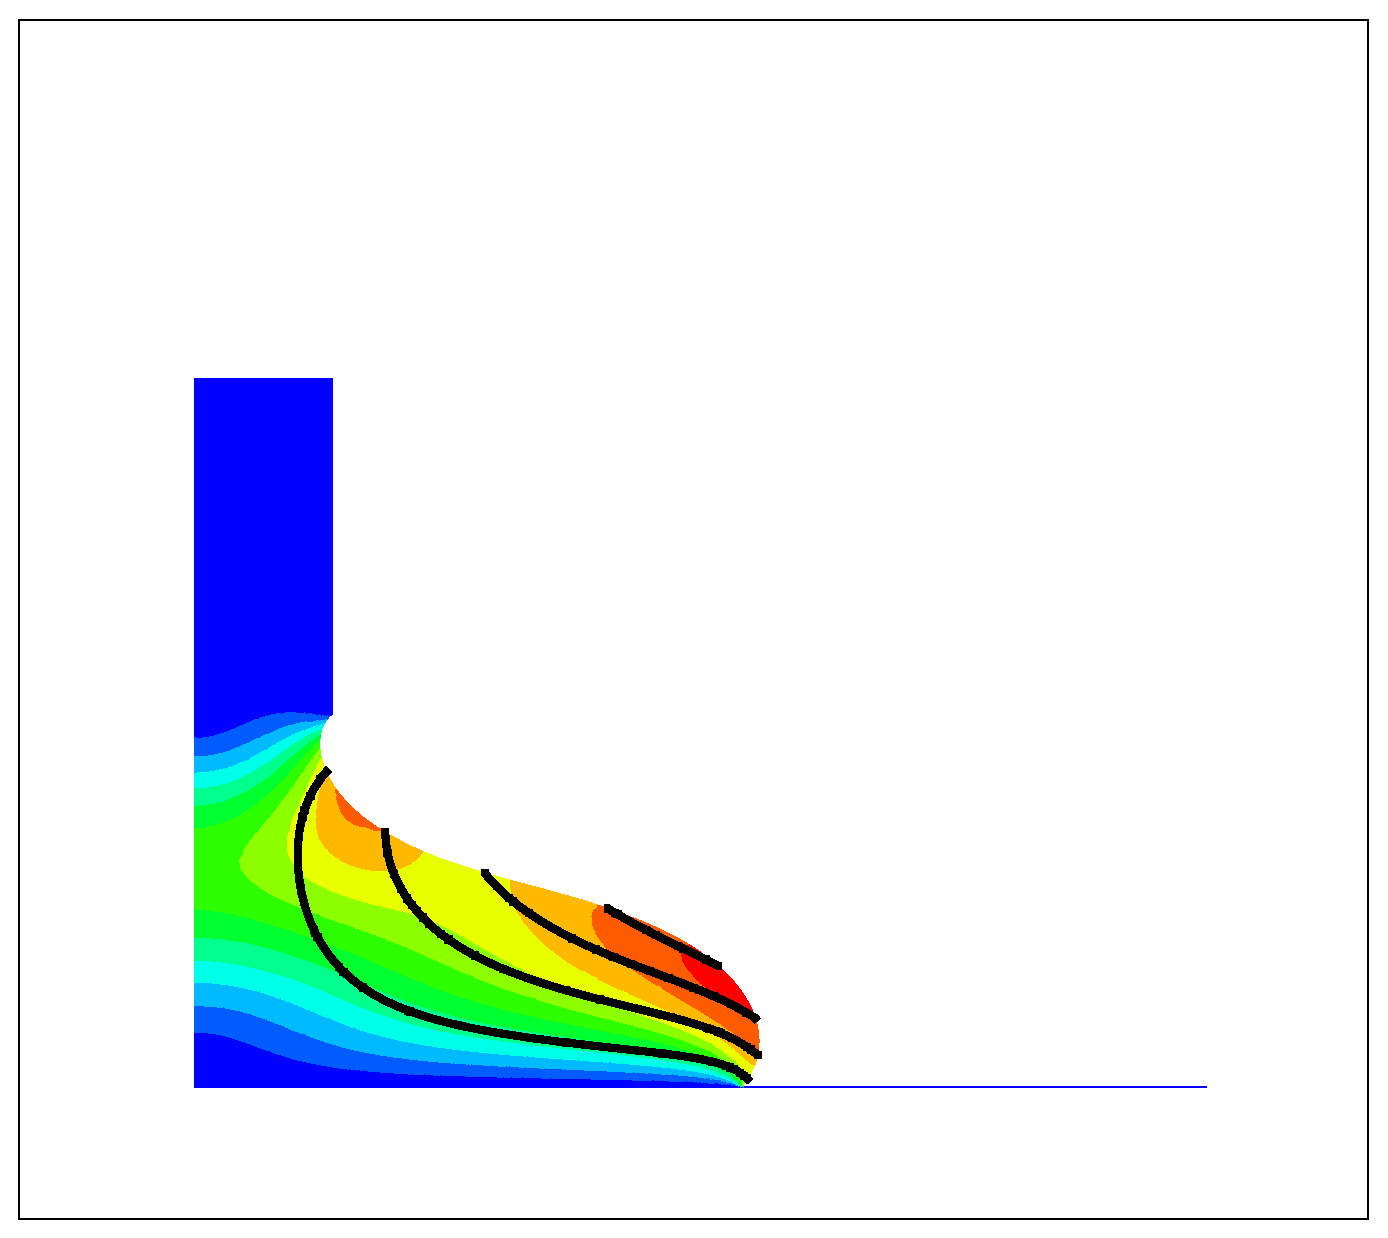
\includegraphics[trim={45px 35px 35px
       35px},clip,width=3.2cm]{figures/glucose_layer_0_0125mm_84_t_2.eps}
   \rput(-1.0,1.7){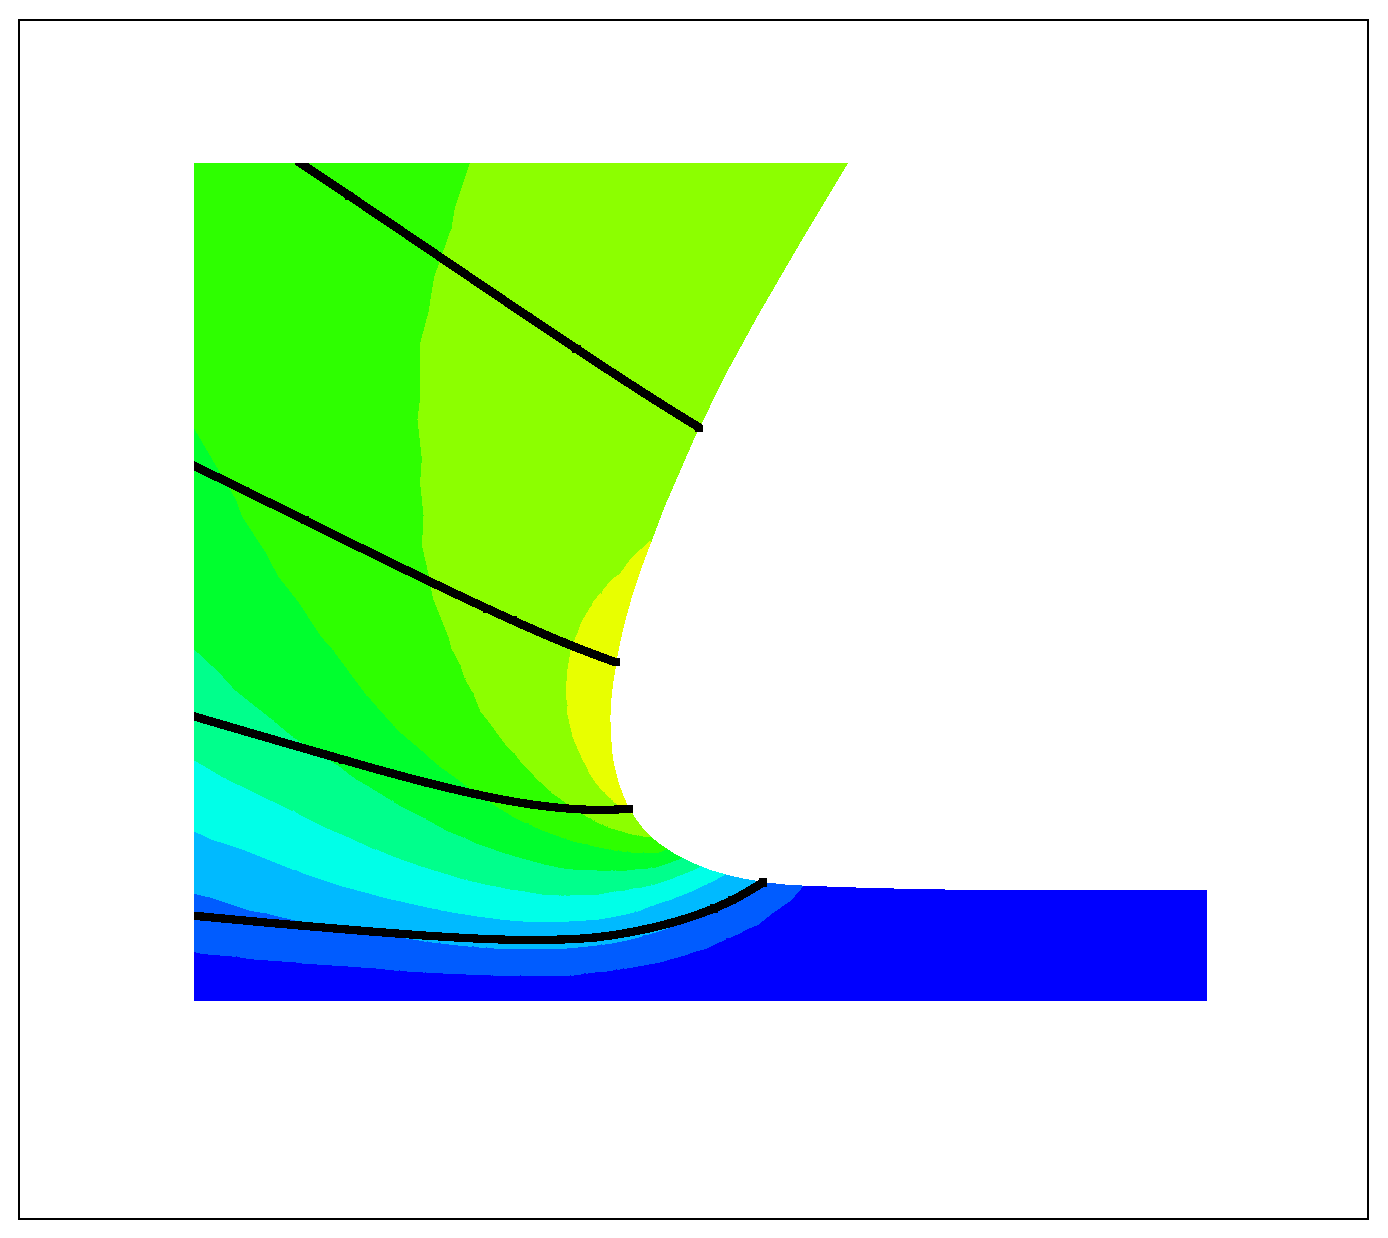
\includegraphics[width=1.75cm]{figures/glucose_layer_0_0125mm_84_t_2_inset2.eps}}
  \end{postscript}
   & 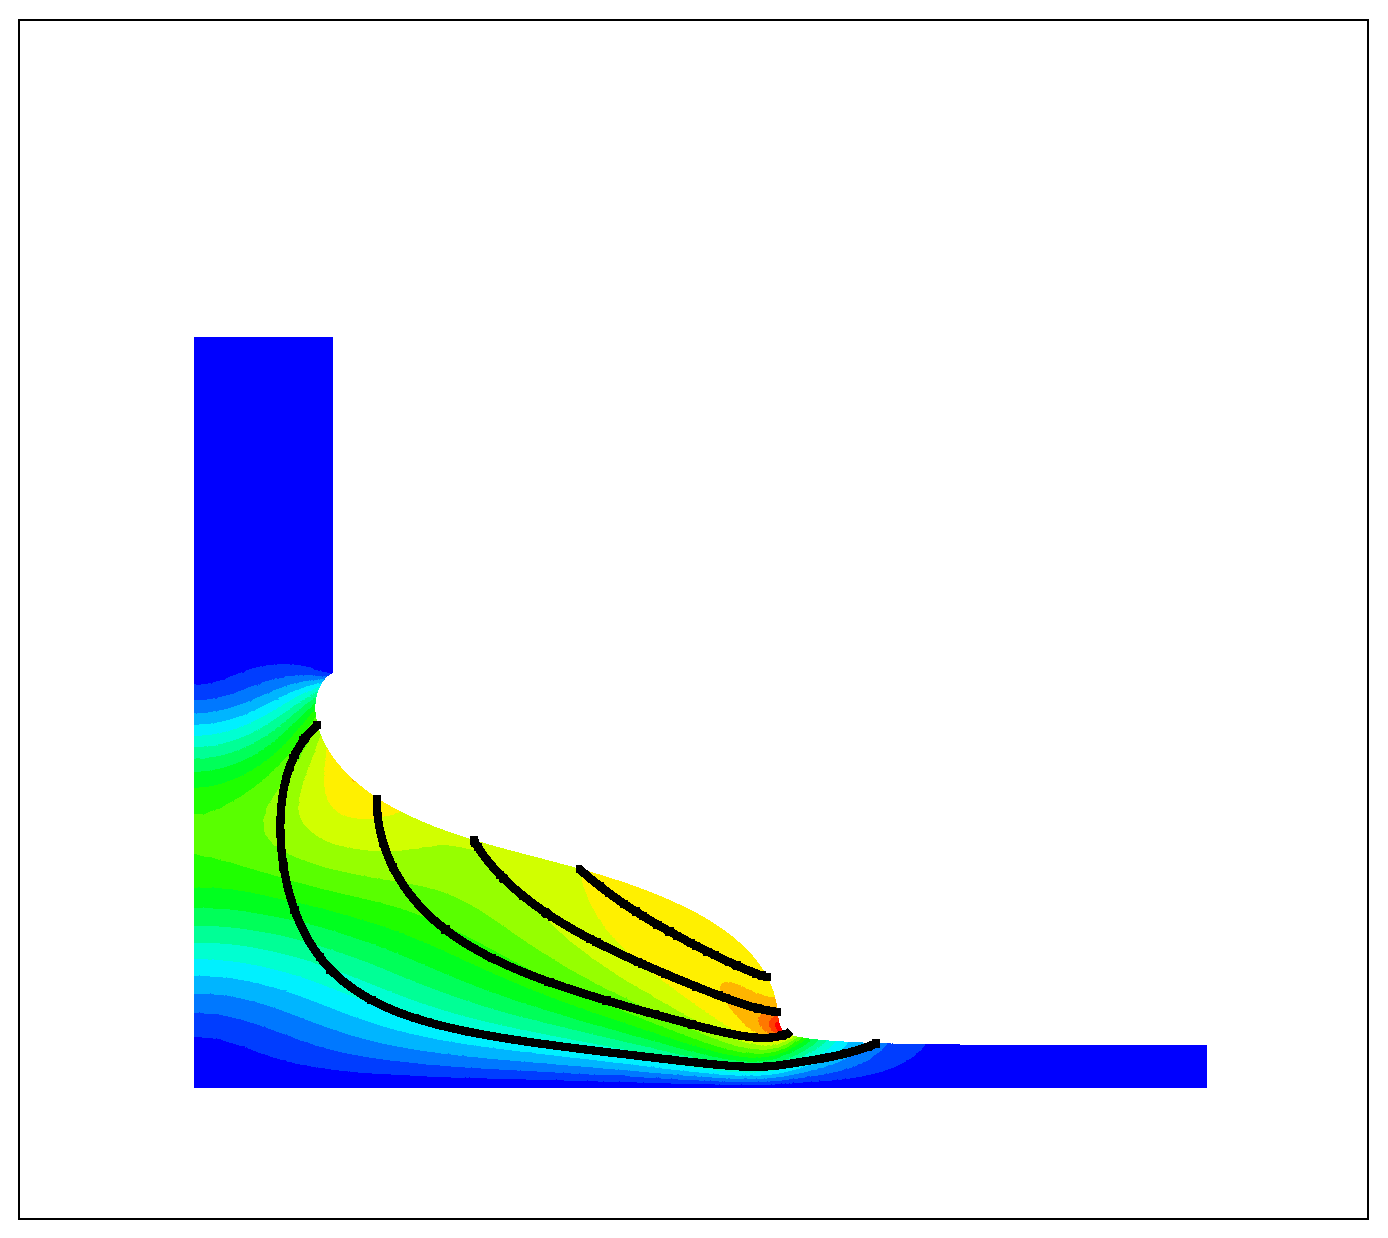
\includegraphics[trim={45px 35px 35px
      35px},clip,width=3.2cm]{figures/glucose_layer_1_25mm_28_t_2.eps}
  & 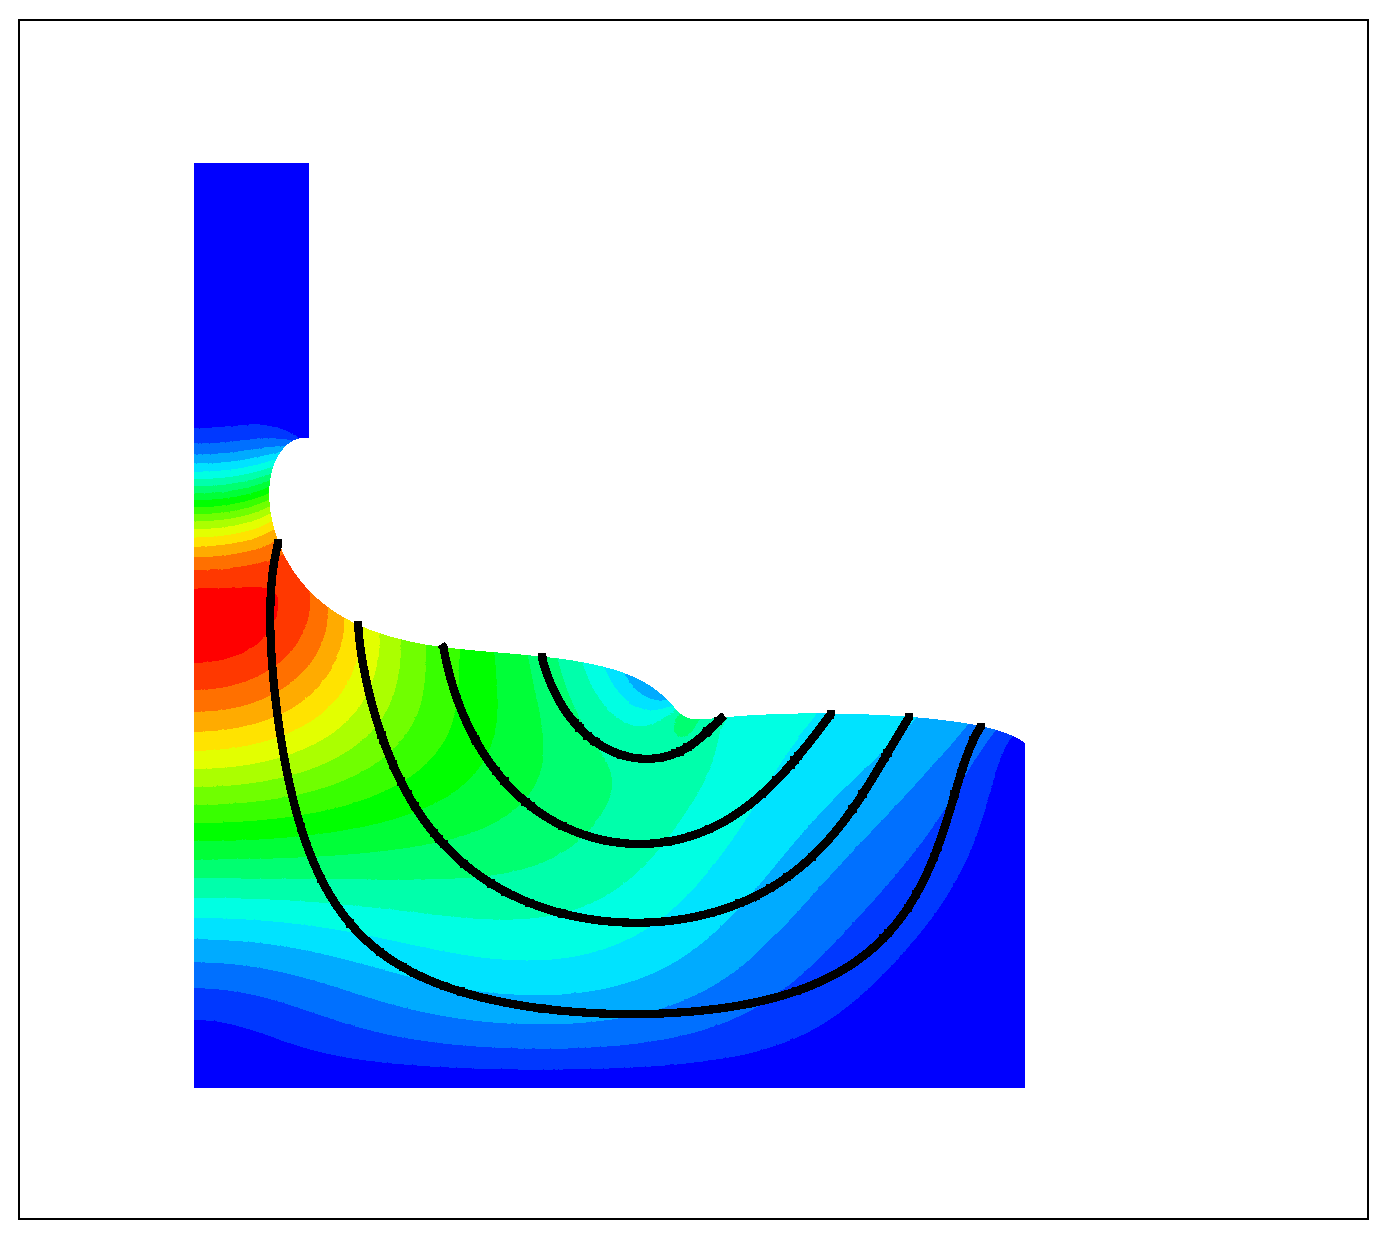
\includegraphics[trim={45px 35px 35px
      35px},clip,width=3.2cm]{figures/glucose_layer_12_5mm_32_t_2.eps}
  \\ \hline 4 & 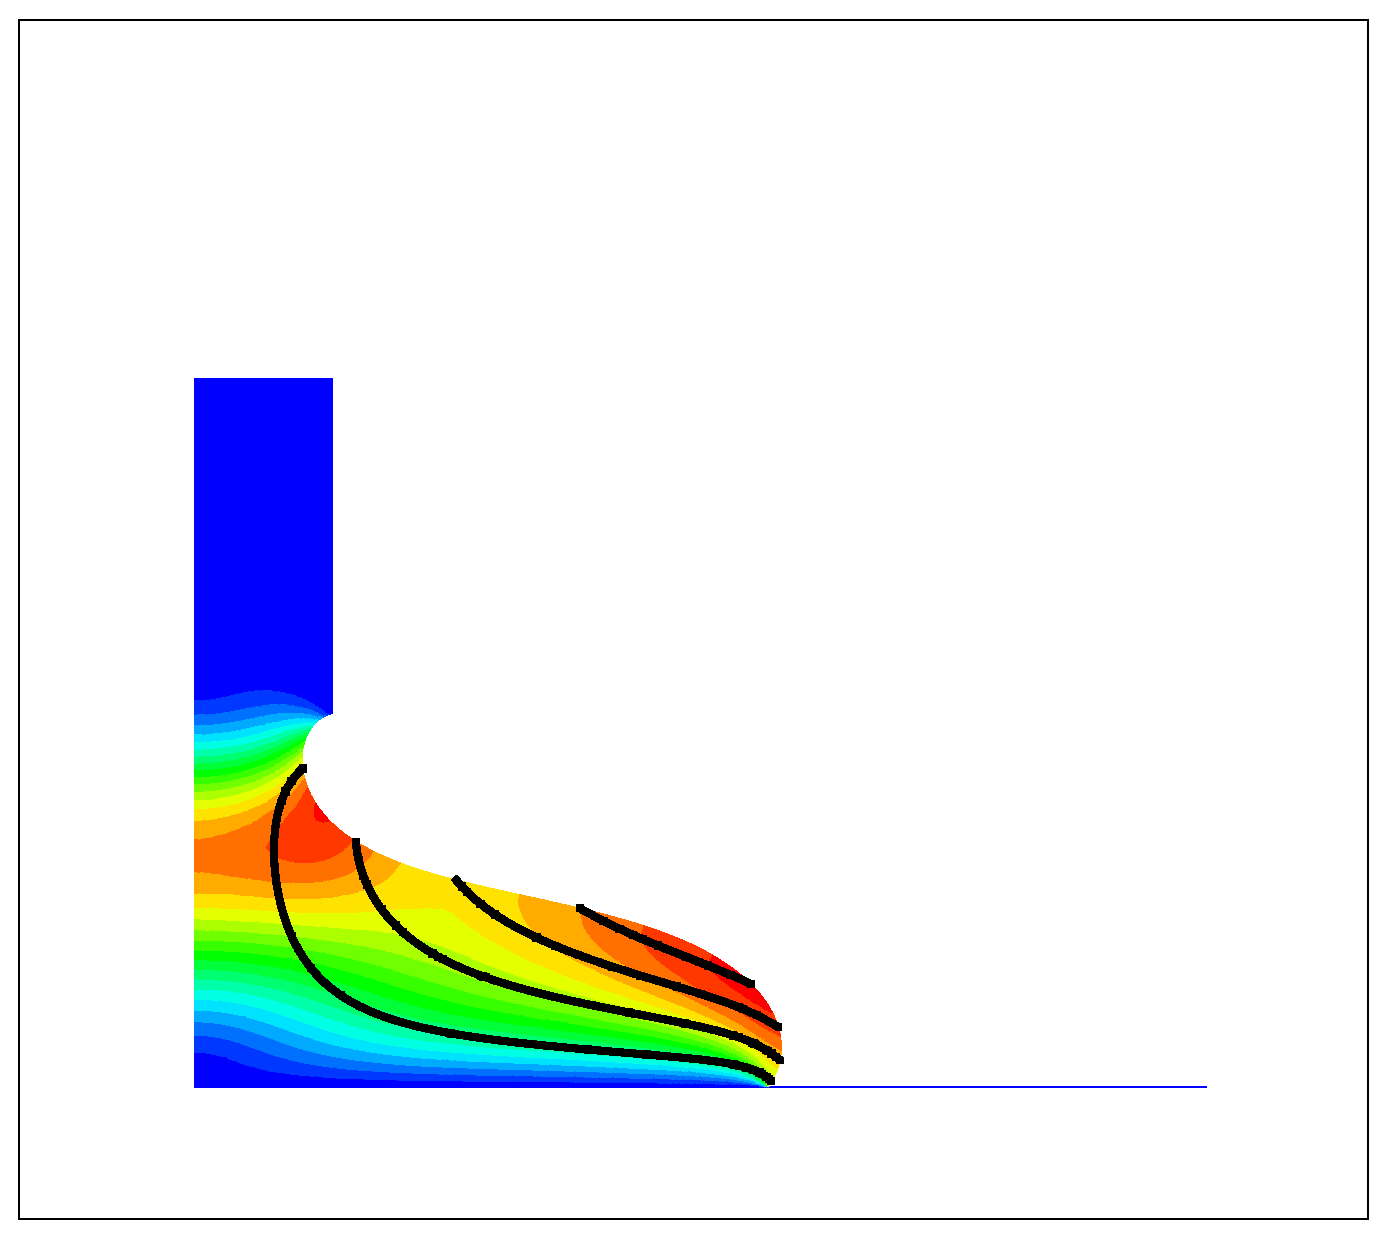
\includegraphics[trim={45px 35px 35px
      35px},clip,width=3.2cm]{figures/glucose_layer_0_0125mm_277_t_4.eps}
  & 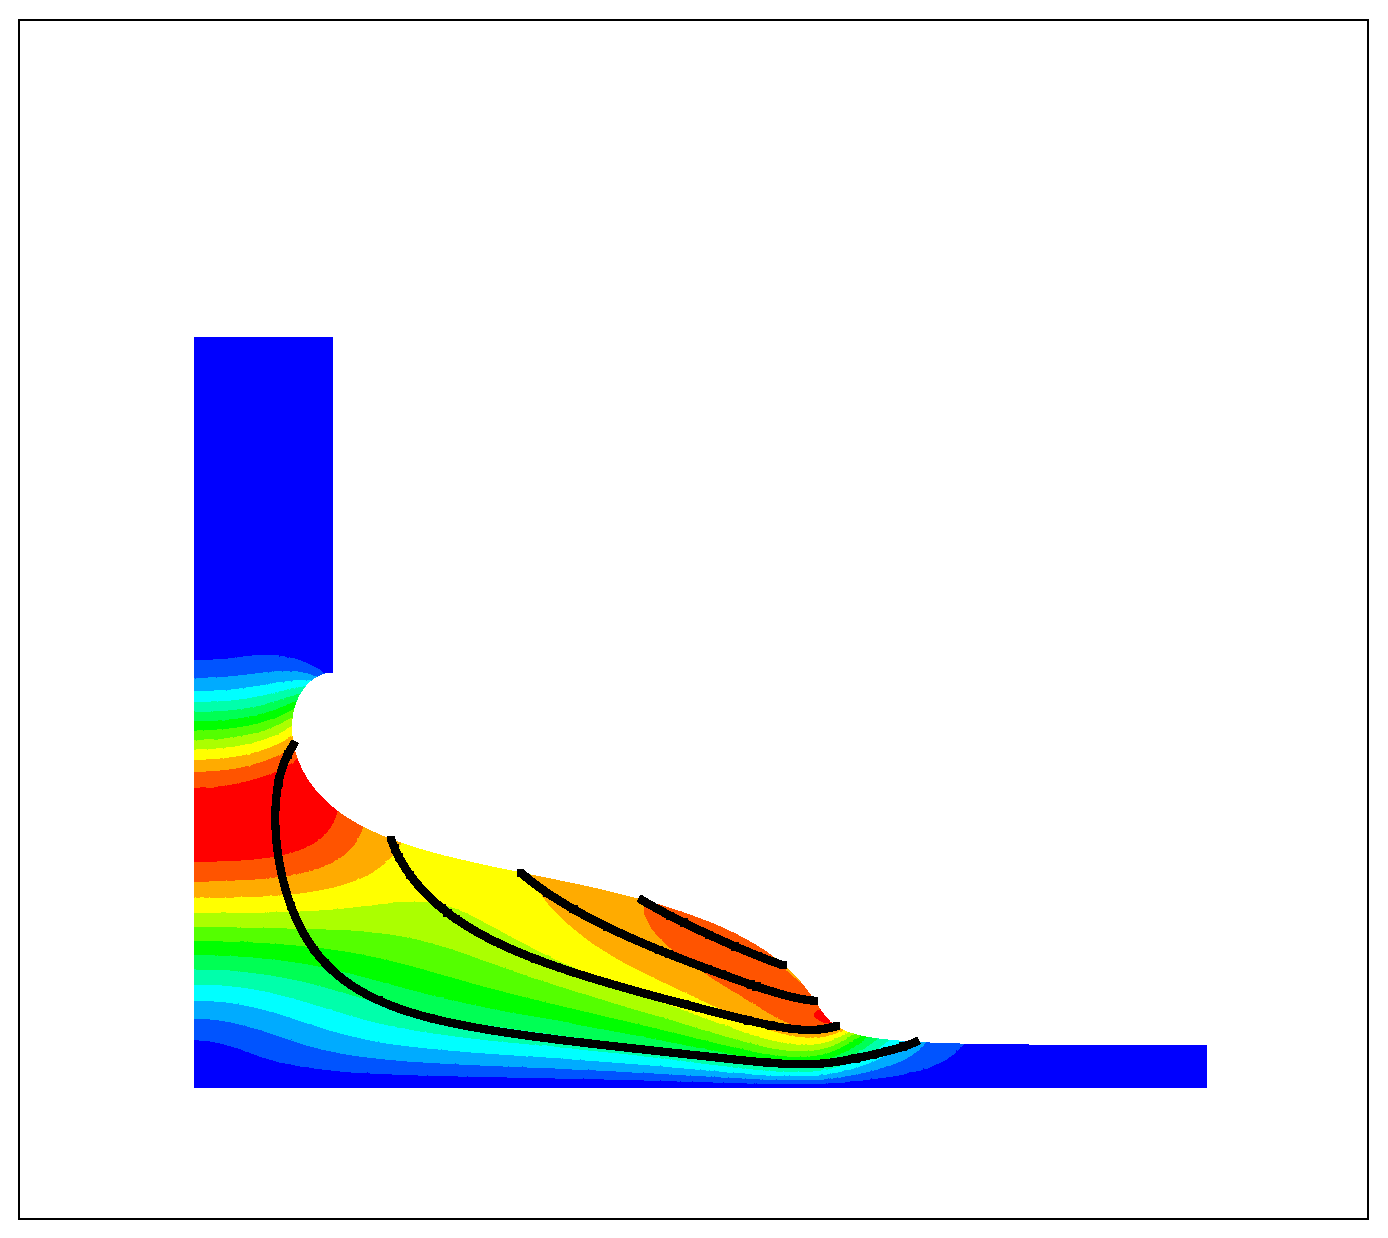
\includegraphics[trim={45px 35px 35px
      35px},clip,width=3.2cm]{figures/glucose_layer_1_25mm_57_t_4.eps}
  & 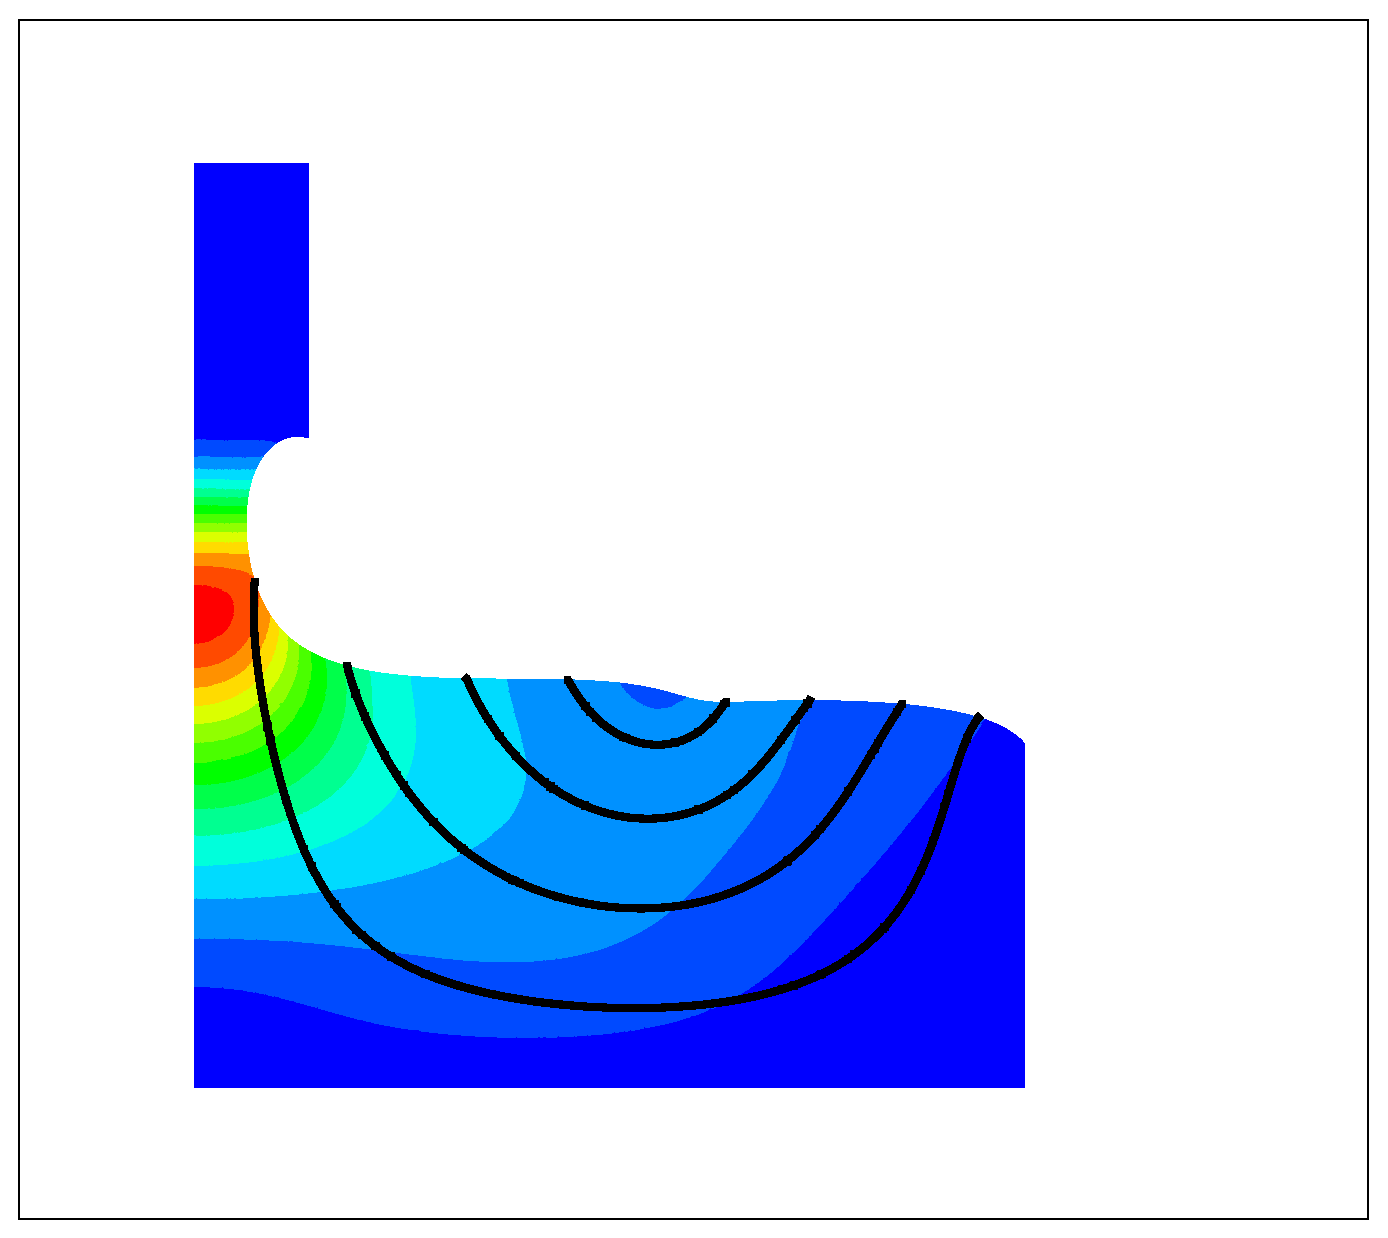
\includegraphics[trim={45px 35px 35px
      35px},clip,width=3.2cm]{figures/glucose_layer_12_5mm_60_t_4.eps}
  \\ \hline 20 & 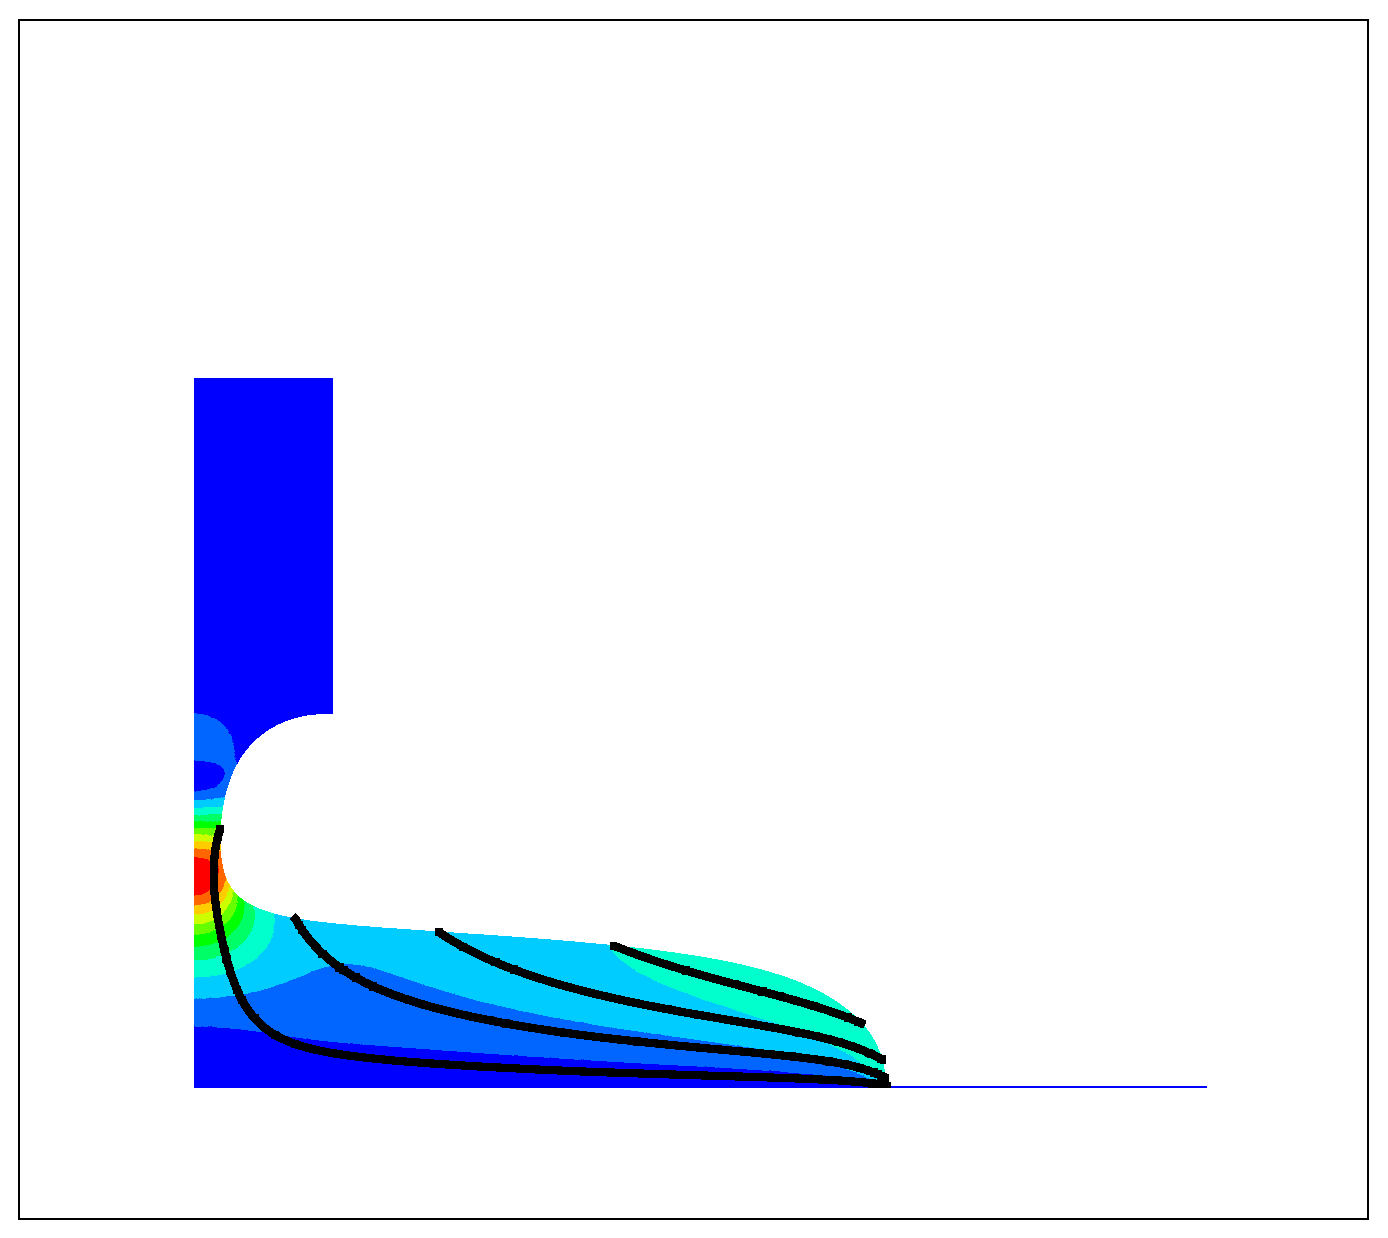
\includegraphics[trim={45px 35px 35px
      35px},clip,width=3.2cm]{figures/glucose_layer_0_0125mm_893_t_20.eps}
  & 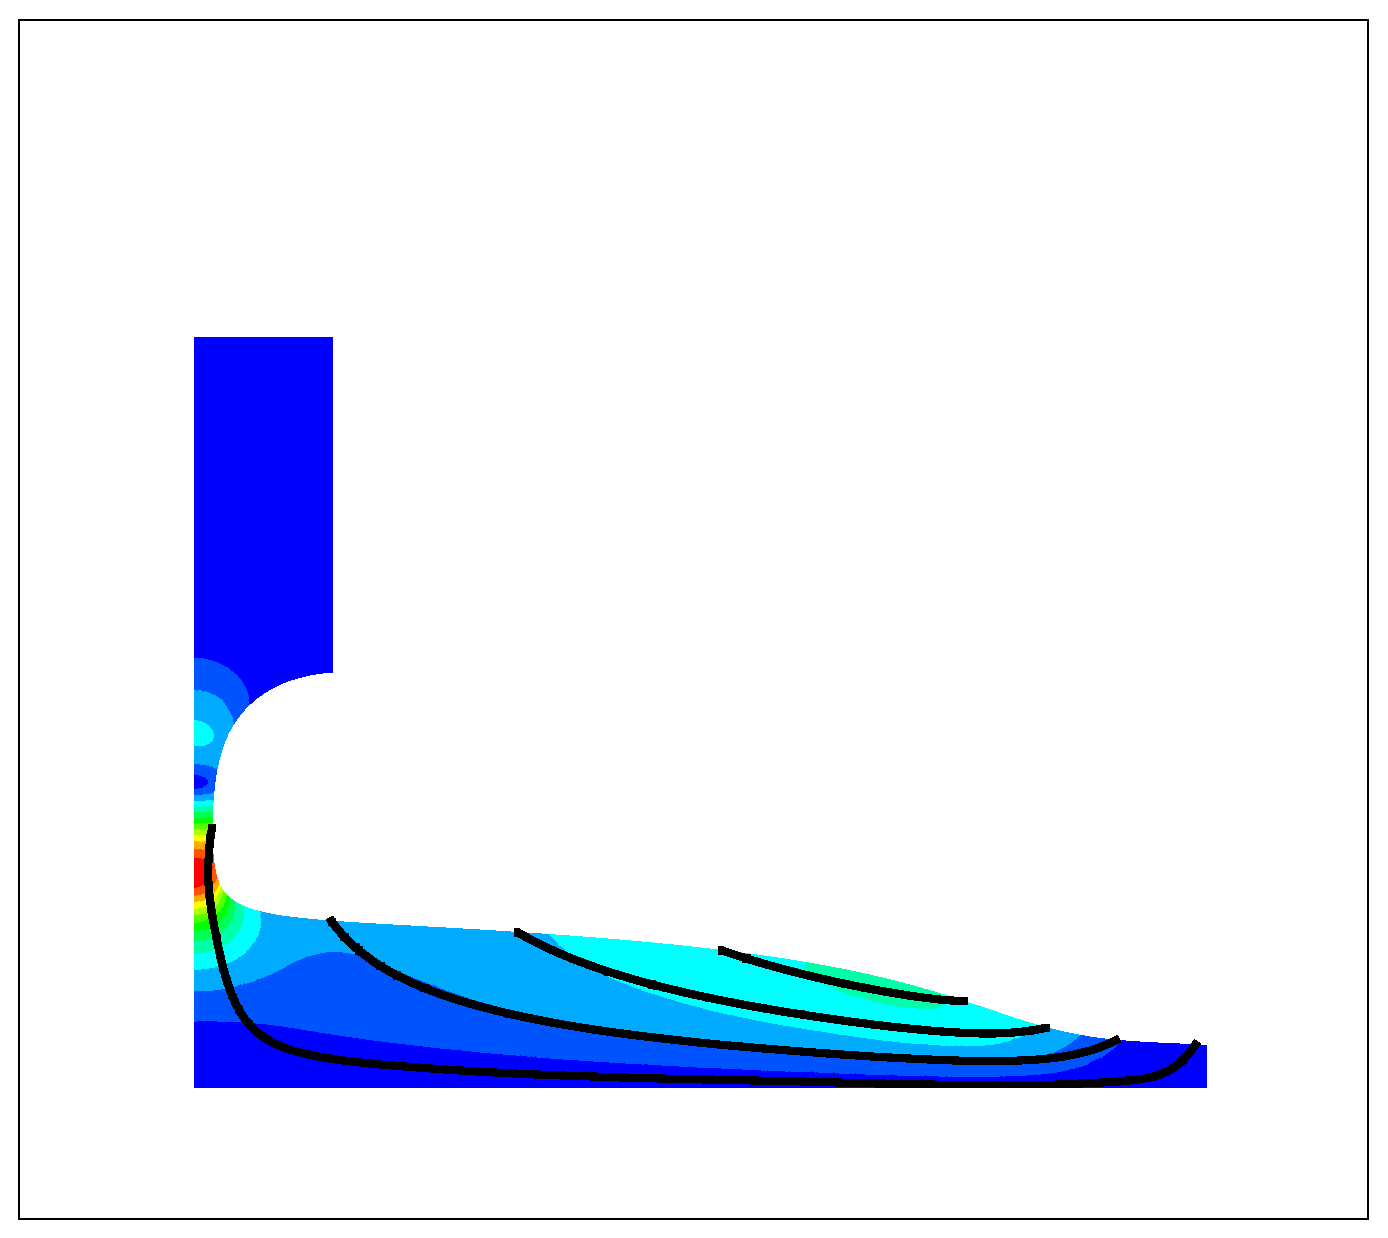
\includegraphics[trim={45px 35px 35px
      35px},clip,width=3.2cm]{figures/glucose_layer_1_25mm_281_t_20.eps}
  & 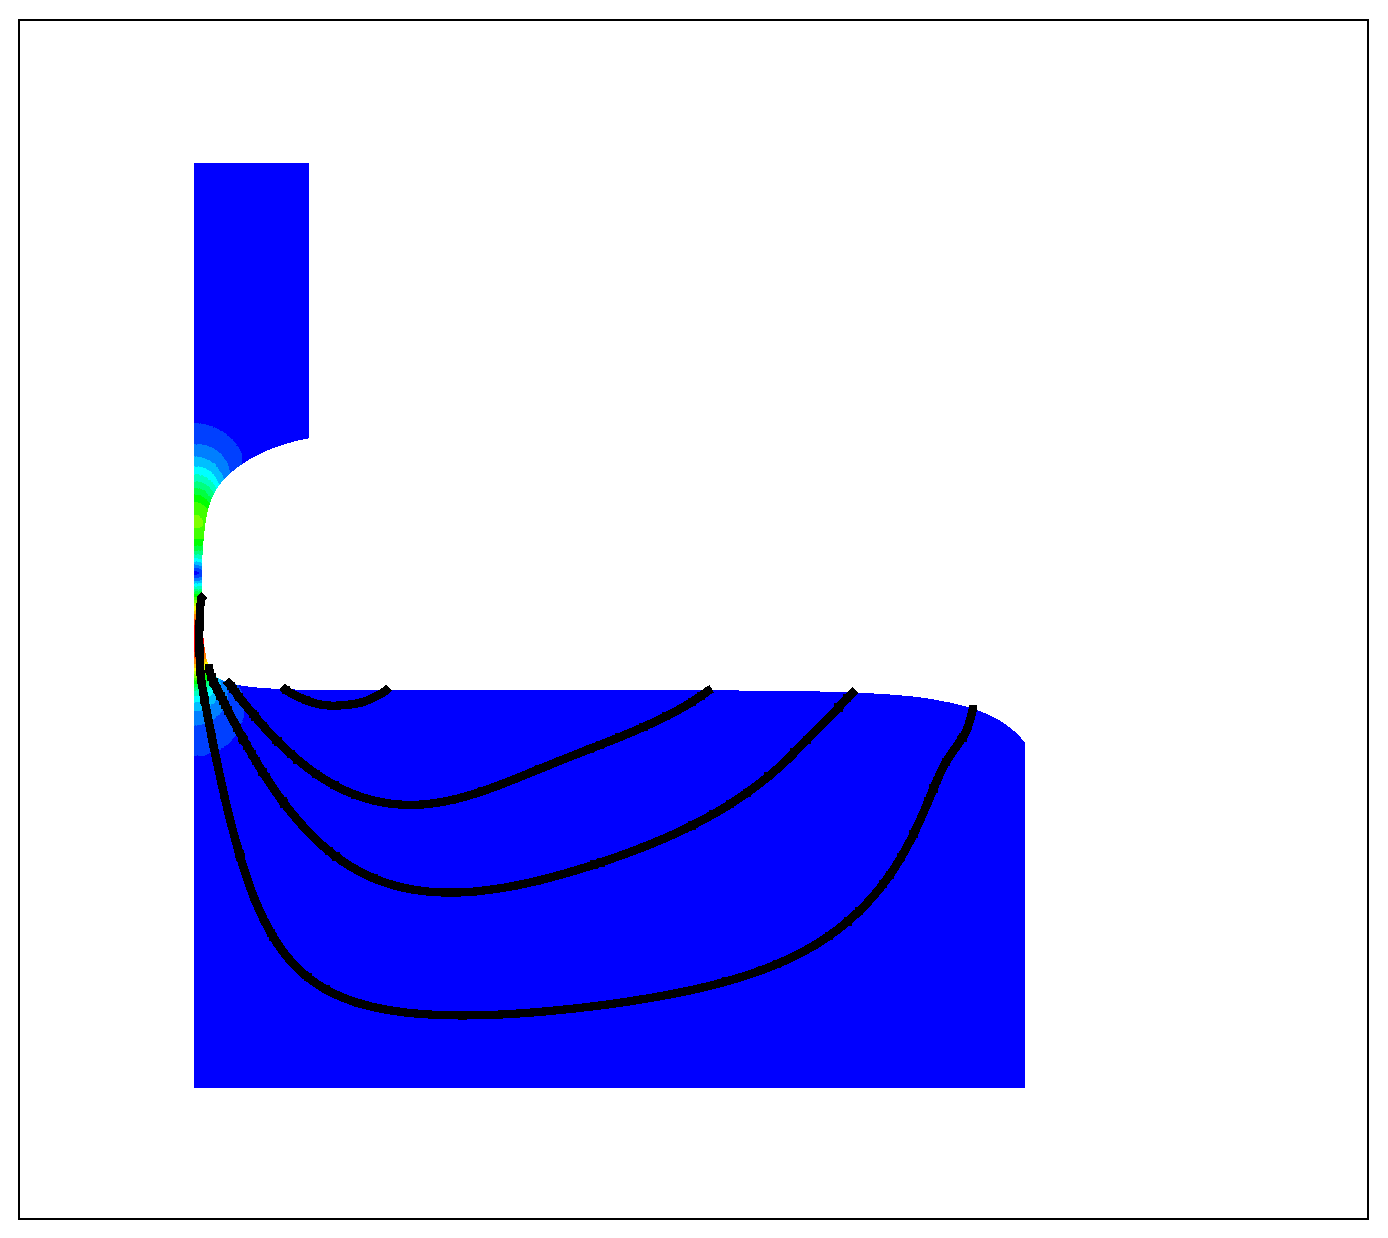
\includegraphics[trim={45px 35px 35px
      35px},clip,width=3.2cm]{figures/glucose_layer_12_5mm_285_t_20.eps}
  \\
 \end{tabular}
 \caption{Illustration of different spreading regimes for different
   layer thicknesses. The contours represent the magnitude of the
   velocity $|u|=\sqrt{u_r^2+u_z^2}$ and the streamlines illustrate
   the velocity field.}
 \label{tab:spreading_regimes}
\end{table}

The same drop spreading on significantly varying layer thicknesses is
illustrated in the sequences in table \ref{tab:spreading_regimes}.
The contours show the magnitude of the flow velocity and the black
lines are representative stream lines.  The rate of spreading as well
as the shape of the drop as it spreads vary significantly depending on
the layer thickness.  For a comparatively thick film of $h^*=12.5$ mm
the stream lines indicate that the drop sinks in.  The flow is
predominantly in the layer, which at $t=2$ results in a bulge of the
free surface ahead of the actual drop contact.  With decreasing layer
thickness there is less flow in the layer and the drop is spreading
instead of sinking in.  However, the spreading mechanism for a layer
thickness of 1.25 mm and 0.0125 mm differs as illustrated in table
\ref{tab:spreading_regimes}.  In case of a layer thickness of 1.25 mm
the drop spreads by fluid flowing into the layer and pushing the free
surface upwards in the contact region, as shown by the stream lines.
This leads to the formation of a wedge, which constantly advances and
is sustained by the flow into the layer ahead.  For a layer thickness
of one hundreth of this value, the fluid no longer flows ahead into
the layer and pushes the interface up.  Instead, the drop spreads
through flow into the contact region which pushes the interface
radially outward. \\


\begin{figure}[!ht]
\centering
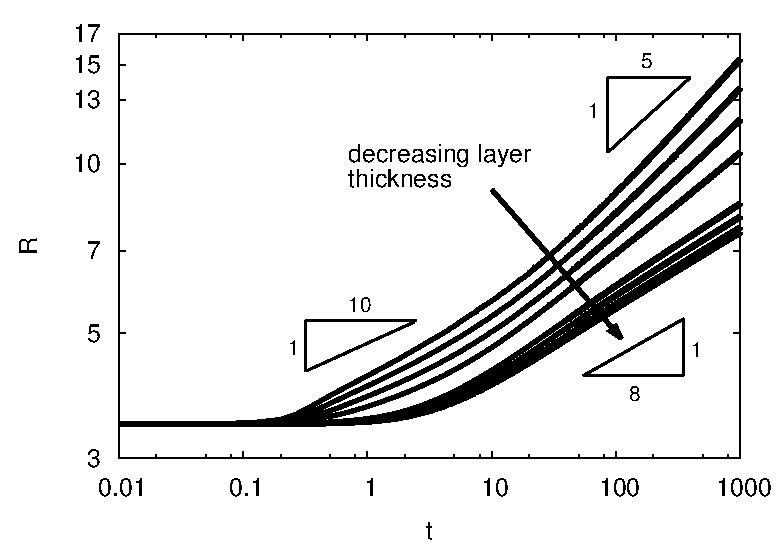
\includegraphics[width=0.6\textwidth]{figures/radius_vs_time_before_and_after_pinch_off.eps}
\caption{Evolution of radius $R$ determined at a 5\% filled gap over
  time for varying layer thicknesses $h^*=1.25, 1.0, 0.75, 0.5, 0.125,
  0.05, 0.0125$ and 0.005 mm.}
\label{fig:radius_vs_time_before_and_after_pinch_off}
\end{figure}

The radius evolution for varying layer thicknesses down to less than
one hundreth of the experimental value is shown in Fig.
\ref{fig:radius_vs_time_before_and_after_pinch_off}.  The results
indicate a transition from one spreading regime to another as the
layer thickness decreases.  In the first regime, covering a layer
thickness $h^*$ from 1.25 to 0.5 mm, the onset of spreading is at
around $t=0.3$.  This onset is followed by surface tension dominated
spreading, indicated by spreading laws of around $R \propto t^{1/10}$.
This spreading mode is followed by viscous dominated spreading with
spreading laws of around $R \propto t^{1/5}$.  The duration of the
initial surface tension spreading reduces with layer thickness and
eventually vanishes for $h^*=0.125$ mm.  In the second regime,
covering a layer thickness $h^*$ from 0.125 to 0.005 mm, the onset of
spreading is at around $t=3.0$ and hence noticably delayed compared to
the first regime.  Also, spreading laws in this regime close to $R
\propto t^{1/8}$ indicate that the entire spreading following onset in
the second regime is dominated by gravity
\cite{cazabat1986dynamics}. \\


In the simulations the liquid thread between the drop and the nozzle
is getting thinner, and this geometric restriction limits the extent
of the computational results.  In order to cover the temporal range in
Fig. \ref{fig:radius_vs_time_before_and_after_pinch_off} we manually
cut this thread and restarted the simulations.  This step can be
performed because Re $\ll$ 1 and inertial effects are negligible.

\begin{figure}[!ht]
\centering
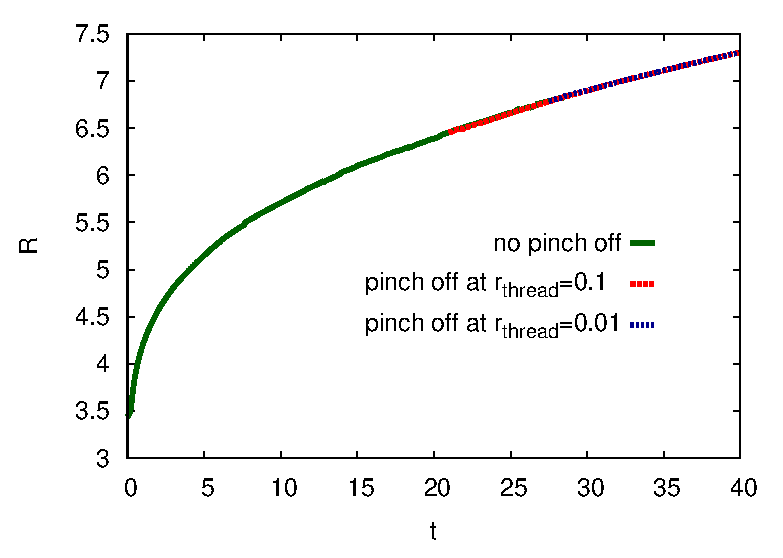
\includegraphics[width=0.6\textwidth]{figures/radius_vs_time_influence_pinch_off.eps}
\caption{Influence of manual for $h^*=1.25$ mm.}
\label{fig:radius_vs_time_influence_pinch_off}
\end{figure}

To assess the influence of when we disconnect the drop from the nozzle
we performed simulations where we cut the thread once its radius
reached a value of $r_{\sym{thread}}=0.1$ and 0.01, respectively.  The
results are shown in Fig.
\ref{fig:radius_vs_time_influence_pinch_off}, where the radius
evolution for the two cases is compared againt the results without
pinch off.  There is excellent agreement in all cases, so therefore we
arbitrarily chose to disconnect at a thread radius of 0.1 and continue
the simulations. \\

\begin{figure}[!ht]
\centering
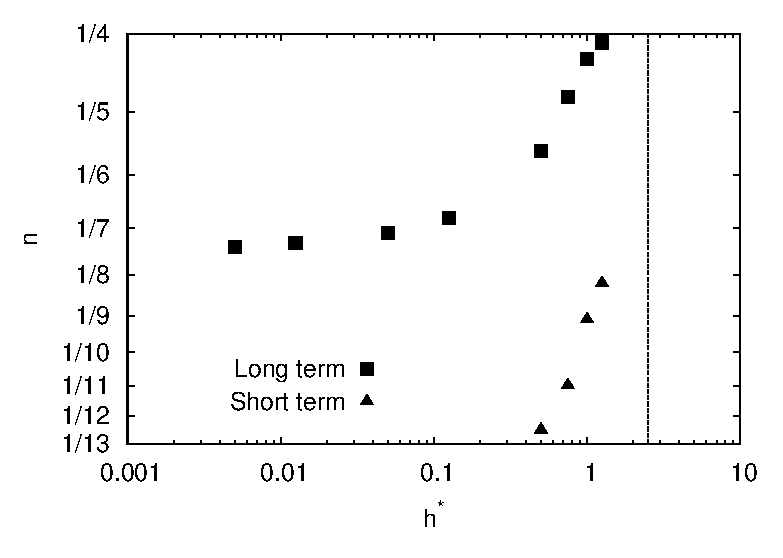
\includegraphics[width=0.6\textwidth]{figures/scaling_vs_layer_inc_short_time.eps}
\caption{Spreading exponent $n$ as function of layer thickness $h^*$
  on a log-log scale for both the short term and long term behaviour.}
\label{fig:scaling_vs_layer}
\end{figure}

From Fig. \ref{fig:radius_vs_time_before_and_after_pinch_off} we
extracted radius scaling laws for both the short term and long term
behaviour.  The different spreading exponents are shown in Fig.
\ref{fig:scaling_vs_layer} as function of the layer thickness.  Only
for layer thicknesses of $h^*=0.5 - 1.25$ mm we were able to extract
a distinct short term scaling, as discussed previously.  The dashed
line indicates a layer thickness of 2.5 mm at which the drop begins to
sink into the layer, similarly to the behaviour observed for
$h^*=12.5$ mm in table \ref{tab:spreading_regimes}.  The spreading
exponents for the long term behaviour in Fig.
\ref{fig:scaling_vs_layer} confirm the existence of two distinct
spreading regimes depending on the layer thickness.  Moreover, they
suggest a smooth transition between these two regimes.  The short
term, surface tension driven spreading evolves with layer thickness
similarly to the long term behaviour. \\


\begin{table}[!ht]
 \centering
 \begin{tabular}{>{\centering\arraybackslash}m{3.5cm}  >{\centering\arraybackslash}m{3.5cm}  >{\centering\arraybackslash}m{3.5cm}}
  \multicolumn{3}{>{\centering\arraybackslash}m{10.5cm}}{$h^*$ in mm}
  \\ 0.005 & 0.125 & 1.25
  \\ 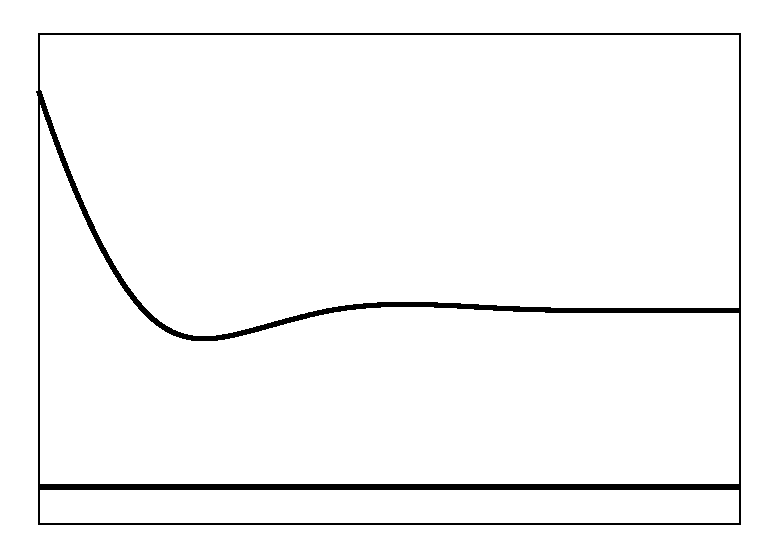
\includegraphics[width=3.2cm]{figures/glucose_layer_0.005mm_free_surface_t_500.eps}
  &
  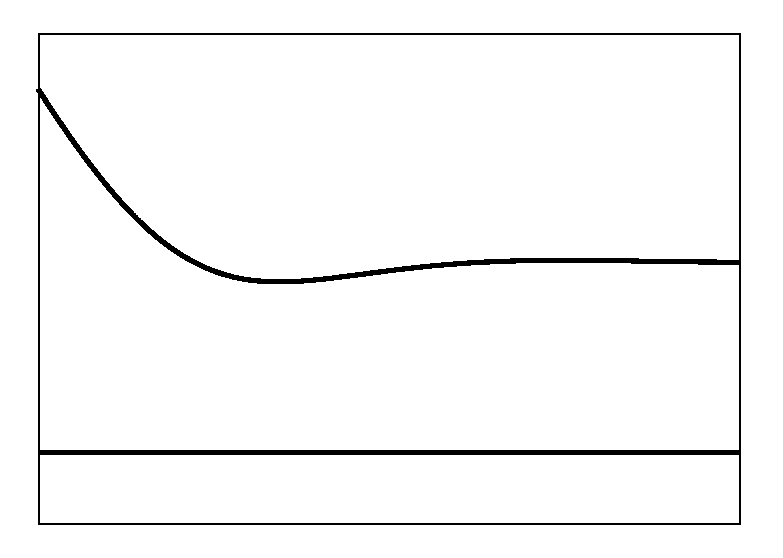
\includegraphics[width=3.2cm]{figures/glucose_layer_0.125mm_free_surface_t_500.eps}
  &
  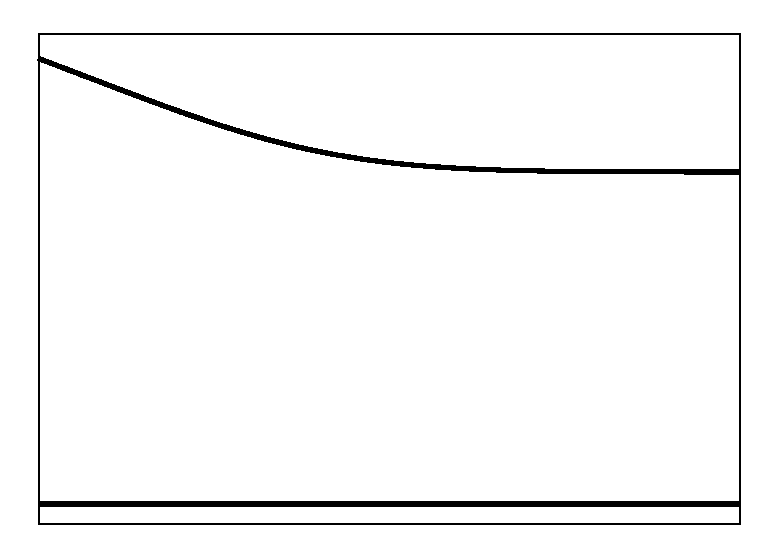
\includegraphics[width=3.2cm]{figures/glucose_layer_1.25mm_free_surface_t_500.eps}
  \\
 \end{tabular}
 \caption{Shape of the propagating front for selected layer
   thicknesses.}
 \label{tab:front_shape}
\end{table}

Typical shapes of the spreading front in an established steady state
propagation, at $t=500$, are shown in table \ref{tab:front_shape}.
For sufficiently thick layers, in this case $h^*=1.25$ mm, there is a
smooth transition from the layer to the drop.  As the layer gets
thinner the Landau-Levich meniscus \cite{maleki2011landau} begins to
form and the thinner the layer the more pronounced it becomes.
However, a direct comparison to Landau and Levich's theory is not
possible, because it is derived for a plate that is withdrawn from a
fluid bath.  Their controlling parameter was the speed of the plate,
equivalent to our spreading velocity here, and their measured quantity
was the residual fluid layer on the plate.  However, in our setup we
impose the thickness of the layer instead of treating it as an
unknown, and hence Landau and Levich's scaling cannot be applied.


\section{Discussion}
TO BE WRITTEN\\
Key findings

\begin{itemize}
 \item spreading on layer viscously dominated, spreading on solid
   surface tension dominated
 \item spreading on layer, exponent dependent on layer thickness
 \item distinct regimes with or without Landau-Levich meniscus
\end{itemize}


% If in two-column mode, this environment will change to single-column format so that long equations can be displayed. 
% Use only when necessary.
%\begin{widetext}
%$$\mbox{put long equation here}$$
%\end{widetext}

% Figures should be put into the text as floats. 
% Use the graphics or graphicx packages (distributed with LaTeX2e).
% See the LaTeX Graphics Companion by Michel Goosens, Sebastian Rahtz, and Frank Mittelbach for examples. 
%
% Here is an example of the general form of a figure:
% Fill in the caption in the braces of the \caption{} command. 
% Put the label that you will use with \ref{} command in the braces of the \label{} command.
%
% \begin{figure}
% \includegraphics{}%
% \caption{\label{}}%
% \end{figure}

% Tables may be be put in the text as floats.
% Here is an example of the general form of a table:
% Fill in the caption in the braces of the \caption{} command. Put the label
% that you will use with \ref{} command in the braces of the \label{} command.
% Insert the column specifiers (l, r, c, d, etc.) in the empty braces of the
% \begin{tabular}{} command.
%
% \begin{table}
% \caption{\label{} }
% \begin{tabular}{}
% \end{tabular}
% \end{table}

% If you have acknowledgments, this puts in the proper section head.
%\begin{acknowledgments}
% Put your acknowledgments here.
%\end{acknowledgments}

% Create the reference section using BibTeX:
\bibliography{glucose_references}

\end{document}
%
% ****** End of file aiptemplate.tex ******
